\documentclass{article}
\usepackage[a4paper, top=2cm, bottom=3cm]{geometry}

\usepackage[ngerman]{babel}
\usepackage{csquotes}

\usepackage{booktabs}

\usepackage{amssymb}
\usepackage{amsmath}
\usepackage{cancel}
\usepackage{mathtools}
\usepackage{enumitem}

\usepackage{hyperref}

\usepackage{graphicx}
\usepackage{wrapfig}
\usepackage{minted}

\usepackage{parskip}
\usepackage{fancyhdr}
\usepackage{vmargin}

\usepackage{pgfplots}
\pgfplotsset{compat=newest}
\usetikzlibrary{external}
\tikzexternalize[prefix=tikz/]

\usepackage{siunitx}
\sisetup{locale = DE}

\usepackage{biblatex}
\DefineBibliographyStrings{ngerman}{
  urlseen = {Abruf vom}
}
\addbibresource{quellen.bib}

\newcommand{\proofeq}{\overset{!}{=}}
\newcommand{\proofeqv}{\overset{!}{\Leftrightarrow}}
\newcommand{\equivalent}{\overset{\scriptscriptstyle\wedge}{=}}
\DeclarePairedDelimiter\ceil{\lceil}{\rceil}
\DeclarePairedDelimiter\floor{\lfloor}{\rfloor}

\date{25.03.2022}
% Physikalisches Grundpraktikum I \\ (Mechanik und Thermodynamik)
\title{Versuch 1: Mechanische Schwingungen}
\author{Finn Bietz (8104485) \\ Wafaa Al Nachwati (8102531) \\ Finn Wagner (8102237)}

\begin{document}

    \makeatletter
\let\thetitle \@title{}
\let\theauthor \@author{}
\let\thedate \@date{}
\makeatother

\fancyhf{}

    \begin{titlepage}
        \centering
        \vspace*{0.5 cm}
        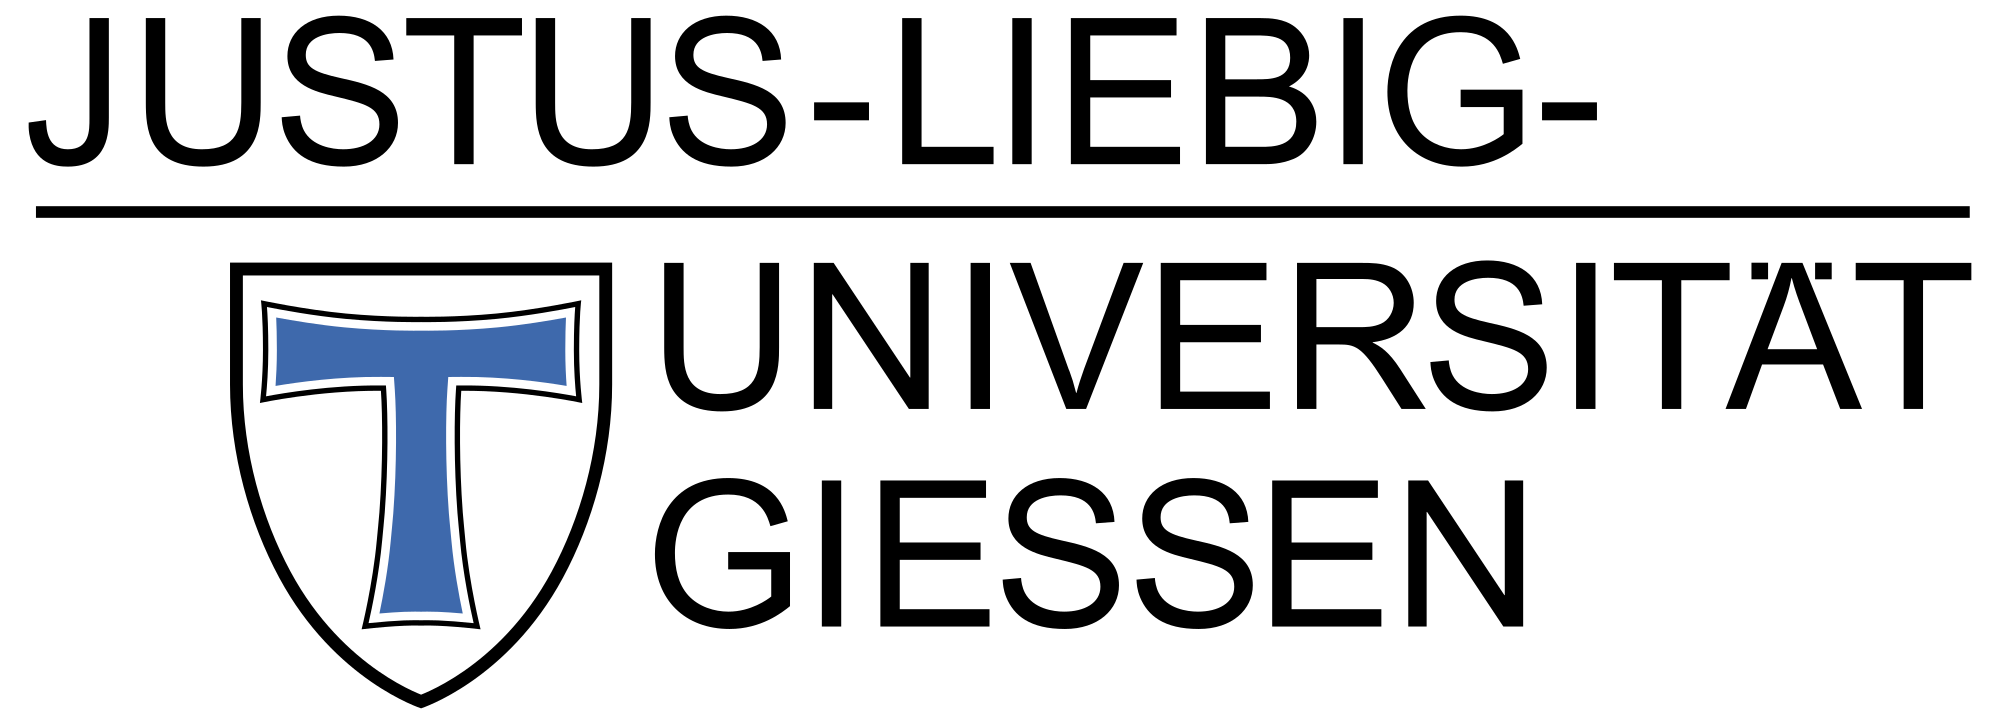
\includegraphics[ width = 0.6 \textwidth ]{fotos/uni-logo.png} \\ [2.0 cm]

        Protokoll zu: \\
        \begin{center}    
            \textsc{ \Large Physikalisches Grundpraktikum I \\ (Mechanik und Thermodynamik)} \\ [2.0 cm]
        \end{center}
        
        \rule{\linewidth}{0.2 mm} \\ [0.4 cm]
        { \huge \bfseries \thetitle} \\
        \rule{\linewidth}{0.2 mm} \\ [1.5 cm]
                
        \begin{minipage}{ 0.4 \textwidth }
            \begin{flushright} \large
                \emph{Protokoll von: } \\
                \theauthor{}
            \end{flushright}
        \end{minipage} \\ [2 cm]
        
    \end{titlepage}

    \section{Versuchsziel und Versuchsmethode}
      In dieser Versuchsreihe mit drei Versuchen beschäftigen wir uns mit Federn und dem Hookeschen Gesetz und Federkonstanten,
      sowie harmonischen Oszillatoren und Schwebungen. \\
      Im ersten Versuch bestimmen wir eine Federkonstante durch mehrere Messungen wie weit die Feder bei einer durch eine Masse
      erzeugten Kraft ausgelenkt wird.
      Im zweiten Versuch betrachten wir einen harmonischen Oszillator. Er besteht aus einem zwischen zwei Federn eingespannten Gleiter.
      Aus der Schwingungsdauer des Gleiters berechnen wir seine Masse.
      Da der Gleiter gedämpft ist messen wir auch die Zeit die es braucht bis die Amplitude der Schwingung auf die Hälfte zurückgegangen ist.
      Aus dieser Zeit berechnen wir die Dämpfungskonstante \(b\). \\
      Für den letzten Versuch fügen wir noch einen weiteren über eine Feder mit geringer Federkonstante verbundenen Gleiter hinzu.
      Wir vermessen die beiden Eigenmoden des Systems und und vergleichen sie mit dem theoretischen Wert.
      Neben den Eigenmoden messen wir auch noch die Schwebungsfrequenz des Systems und vergleichen auch diese mit unseren theoretischen Vorhersagen.

    \section{Allgemeiner Aufbau}
      Die Experimente in diesem Versuch, werden um Reibungseffekte zu minimieren und das messen zu erleichtern auf einer Luftkissenbahn durchgeführt.
      % TODO: FOTO
      Zur genaueren Auswertung verwenden wir eine digitale Messapparatur. Sie misst mit einer CCD-Kamera über eine reflektierende Folie am Gleiter deren Position.

    \section{Bestimmung der Federkonstanten}
      \subsection{Theorie}
          Wenn eine Feder gedehnt wird besteht ein linearer Zusammenhang zwischen der Kraft $F_k$, mit welcher die Feder in Richtung die Ausgangslage zieht. Die Federkraft ist gegeben als:
          \begin{equation}
              F_k = -kx
          \end{equation}
          Wobei $x$ die Auslenkung aus der Ruhelage und $k$ die Federkonstante  ist.\\
          Um nun die Federkonstante zu bestimmen wird ein Kräftegleichgewicht von $F_k$ und der Gewichtskraft $F_G$ von einer Masse, welche an die Feder angehängt wird erzeugt:
          \begin{equation}
              F_k = F_G
          \end{equation}
          Die Gewichtskraft ist gegaben als $F_G = mg$, mit der Masse $m$ und der Gravitationsbeschleunigung $g$, und bei dem Kräftegleichgewicht sind die Beträge gleich:
          \begin{equation}
              kx = mg
          \end{equation}
          Formt man die Gleichung um ergibt sich für die Federkonstante:
          \begin{equation}\label{eq:k}
              k = \frac{mg}{x}
          \end{equation}
      \subsection{Versuchsdurchführung}
          \subsubsection{Materialien}
              \begin{itemize}
                  \item Luftkissenbahn
                  \item 2 Federn
                  \item Gleiter
                  \item Schale, angehängt an einer breiten Schnur
                  \item Verschiedene Gewichte mit bekannter Masse
              \end{itemize}
          \subsubsection{Aufbau}
              Die Feder wird zwischen einer festen Aufhängung und dem Gleiter auf der Luftkissenbahn eingehängt, und das andere Ende des Gleiters wird mit der Schale verbunden.
              Die breite Schnur wird über ein Umlenkstück, aus welchem Luft, wie aus der Luftkissenbahn austreten kann gelegt (um die Reibung zu minimieren) und die Schale hängt nun in der Luft.
              \begin{figure}[ht]\label{fig:foto_federkonstante}
                \centering
                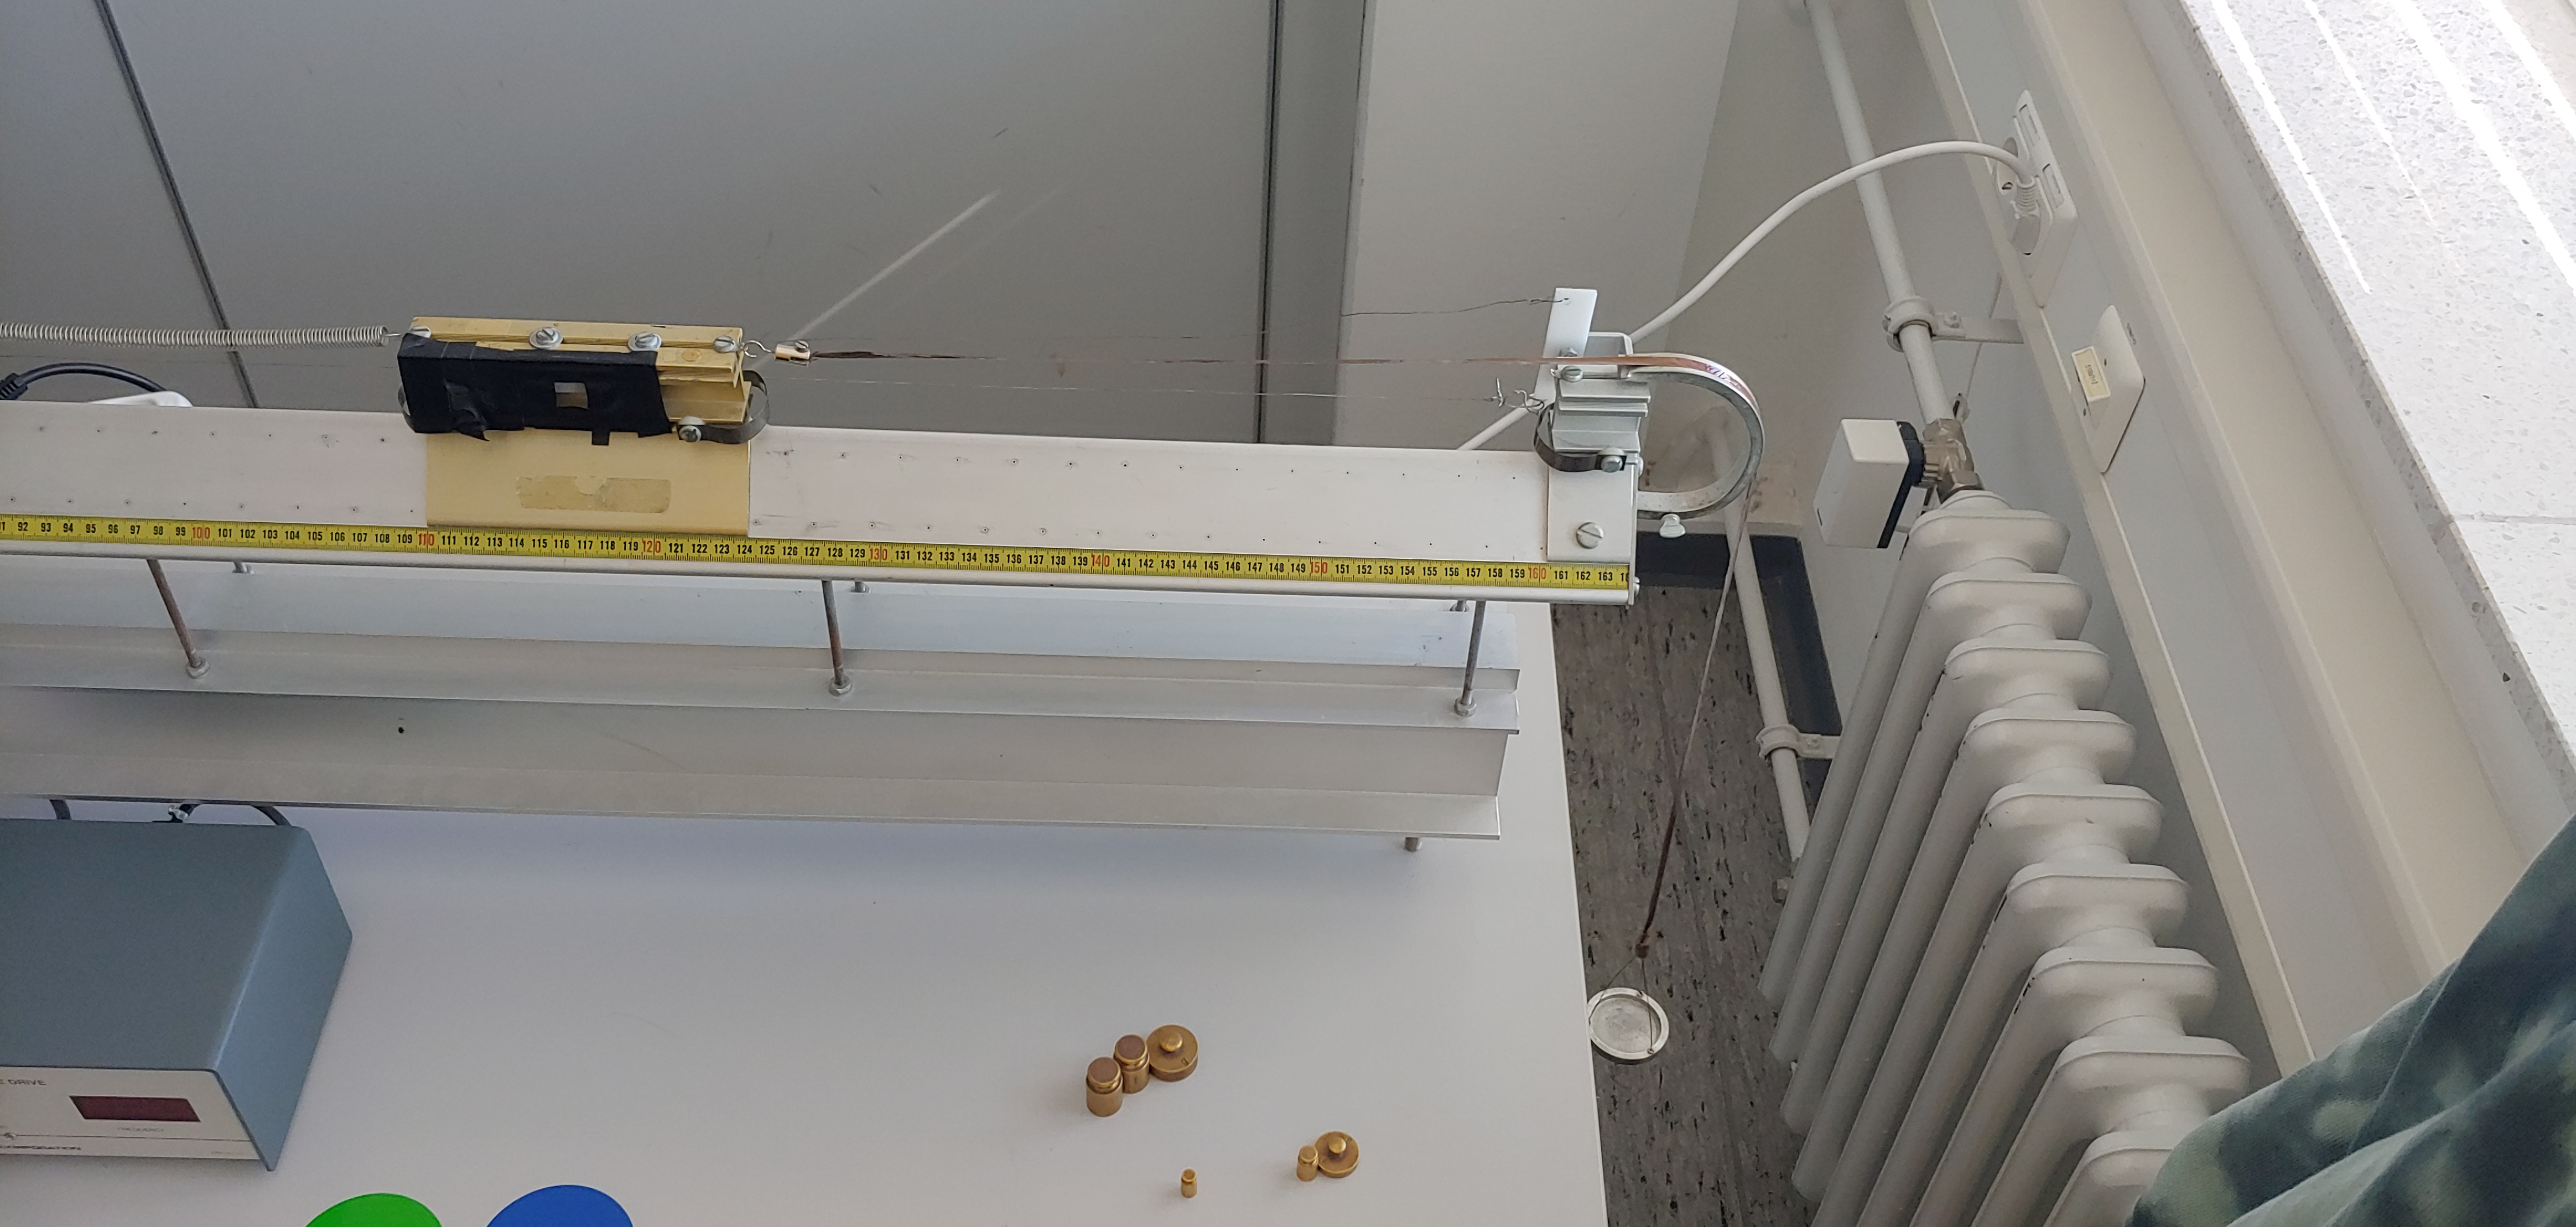
\includegraphics[width=7cm]{fotos/federkonstante.jpg}
                \caption{Foto des Versuchsaufbaus}
            \end{figure}
          \subsubsection{Durchführung}
              Zuerst wird die Ruhelage notiert, an der Luftkissenbahn ist dafür eine cm Skala angebracht.
              Nun wird ein kleines Gewicht in die Schale gelegt, und die neue Position des Gleiters wird notiert.
              Dann werden so Gewichte hinzugefügt und weggenommen, dass die Masse in der Schale ein wenig zunimmt, und die neue Position wird wieder notiert.
              Dies wird wiederholt, bis ungefähr 10 Datenpunkte aufgenommen wurden (oder die Feder nicht weiter gedehnt werden sollte).
              Dies wird jeweils für beide Federn durchgeführt, sodass $k$ und $k^{\prime}$ bestimmt werden können
              

      \subsection{Messergebnisse}
          \subsubsection{Ergebnisse für $k$}
              Für die stärkere Feder mit der Federkonstanten $k$ wurden folgende Messdaten aufgenommen:
              \begin{table}[!h]
                  \centering
                  \begin{tabular}{ | c | c | }
                      \hline
                      Gewicht[g] & Position[cm] \\
                      \hline
                      0          & 110 \\
                      10         & 110,5 \\
                      20         & 111 \\
                      30         & 111,5 \\
                      50         & 112,5 \\
                      60         & 113,1 \\
                      70         & 113,6 \\
                      80         & 114,1 \\
                      100        & 115,1 \\
                      \hline
                  \end{tabular}
                  \caption{Messergebnisse $k$}
              \end{table}

          \subsubsection{Ergebnisse für $k^{\prime}$}
              Und für die Bestimmung der Federkonstanten der schwächeren Feder $k\prime$ wurden folgende Daten gemessen:
              \begin{table}[!h]
                  \centering
                  \begin{tabular}{ | c | c | }
                      \hline
                      Gewicht[g] & Position[cm] \\
                      \hline
                      0          & 104,1 \\
                      5          & 105,6 \\
                      10         & 107,1 \\
                      15         & 108,6 \\
                      20         & 110,1 \\
                      25         & 111,6 \\
                      30         & 113,1 \\
                      35         & 114,6 \\
                      \hline
                  \end{tabular}
                  \caption{Messergebnisse $k^{\prime}$}
              \end{table}
      \subsection{Auswertung}
          Um die Federkonstanten zu bestimmen wird die Position des Gleiters als Funktion der wirkenden Kraft (und damit des angehängten Gewichts) in einem Diagramm eingetragen.
          Da die Gewichtskraft über $mg$ gegeben ist, wird die X-Achse mit Vielfachen von $g$ skaliert.
          Dann wird per Hand eine Gerade an die Punkte gefittet, und die Steigung $S$ der Geraden wird bestimmt.
          Aus der Steigung wird dann die Federkonstante berechnet, sie beträgt $k = \frac{1}{S}$. Der Fehler der Federkonstante wird graphisch bestimmt.

          \subsubsection{Bestimmung von $k$}
              In Abbildung \ref{fig:k} ist der Graph zu $k$ zu sehen.
              Um die Steigung zu bestimmen werden zwei Punkte auf der Geraden ausgewählt, und die Steigung wird mit einem Steigungsdreieck berechnet:\\
              \[P_1:\;\; 0,005kg\cdot g\; ;\; 110,25cm\]
              \[P_2:\;\; 0,125kg\cdot g\; ;\; 115,75cm\]
              So ergibt sich für die Steigung:
              \begin{equation}
                  S = \frac{1,1575m - 1,1025m}{0,125kg\cdot g - 0,005kg\cdot g} = 0,0467 m/N
              \end{equation}
              Nun wird der graphische Fehler von $S$ bestimmt.
              Der Fehler $\Delta S$ ist gegeben als:
              \begin{equation}
                  \frac{\Delta S}{S} = \frac{2\Delta F}{F_2 - F_1}
              \end{equation}
              Und es ergibt sich mit der größten Abweichung $\Delta F$ von der geraden bei $112,5cm$ von $0,001kg\cdot g$:
              \begin{equation}
                  \Delta S = \frac{2\cdot 0,001kg\cdot g}{0,125kg\cdot g - 0,005kg\cdot g}\cdot 0,0497m/N = 0,0007783m/N
              \end{equation}
              Und damit für die Federkonstante:
              \begin{equation}
                  k = \frac{1}{0,0467\pm 0,0007783} = 21,41\substack{+0,36 \\ -0,35}N/m
              \end{equation}

              \begin{figure}[!ht]
                  \centering
                  \includegraphics[width=1\textwidth, angle=270, width=\textwidth]{fotos/k.png}
                  \caption{\label{fig:k}Diagramm von $k$}
              \end{figure}

          \subsubsection{Bestimmung von $k^{\prime}$}
              Es werden wieder zwei Punkte ausgewählt (Abb \ref{fig:kStrich}):
              \[P_1:\;\; 0,0030kg\cdot g\; ;\; 1,05m\]
              \[P_2:\;\; 0,0364kg\cdot g\; ;\; 1,15m\]
              Mit diesen Werten ergibt sich eine Steigung von:
              \begin{equation}
                  S^{\prime} = \frac{1,15m - 1,05m}{0,0364kg\cdot g - 0,003kg\cdot g} = 0,3052 m/N
              \end{equation}
              \begin{figure}[!ht]
                \centering
                \includegraphics[width=1\textwidth, angle=270, width=\textwidth]{fotos/kStrich.png}
                \caption{\label{fig:kStrich}Diagramm von $k^{\prime}$}
            \end{figure}
              Zur Bestimmung des Fehlers wird der Wert, welcher am stärksten von der Grade abweicht genutzt.
              Hier liegen jedoch alle Werte genau auf der Geraden, da die Position des Gleiters nur auf 1mm genau abgelesen werden kann.
              Das führt dazu, dass alle Werte den Gleichen Abstand haben, und daher genau auf einer Geraden liegen.
              Es ergibt sich graphisch also ein Fehler von $0 m/N$, die Messung wird jedoch natürlich nicht komplett fehlerlos sein.\\
              %???
              Und die Federkonstante beträgt damit:
              \begin{equation}
                  k^{\prime} = \frac{1}{0,3052} = 3,28N/m
              \end{equation}

      \subsection{Diskussion}
          Die Methode eignet sich sehr gut zur Bestimmung von Federkonstanten, sie ist leicht durchzuführen und liefert genaue Ergebnisse. Die Reduzierung der Reibung durch die Luftkissenbahn trägt dazu erheblich bei. Mit einer genaueren Skala zur Positionsbestimmung oder längeren Messreihen könnte die Genauigkeit natürlich verbessert werden.

    \section{Gedämpfte harmonische Oszillation}
      \subsection{Durchführung}
          \begin{itemize}
              \item Gleiter auf der Luftkissenbahn zwischen zwei Federn befestigen.
              \item Zeitaufnahme auf den PC starten
              \item Gleiter 5cm in einer Richtung auslenken.
              \item Periodendauer aus dem Graphen ablesen
          \end{itemize}
          \begin{figure}[!ht]\label{fig:foto_harmonisch}
              \centering
              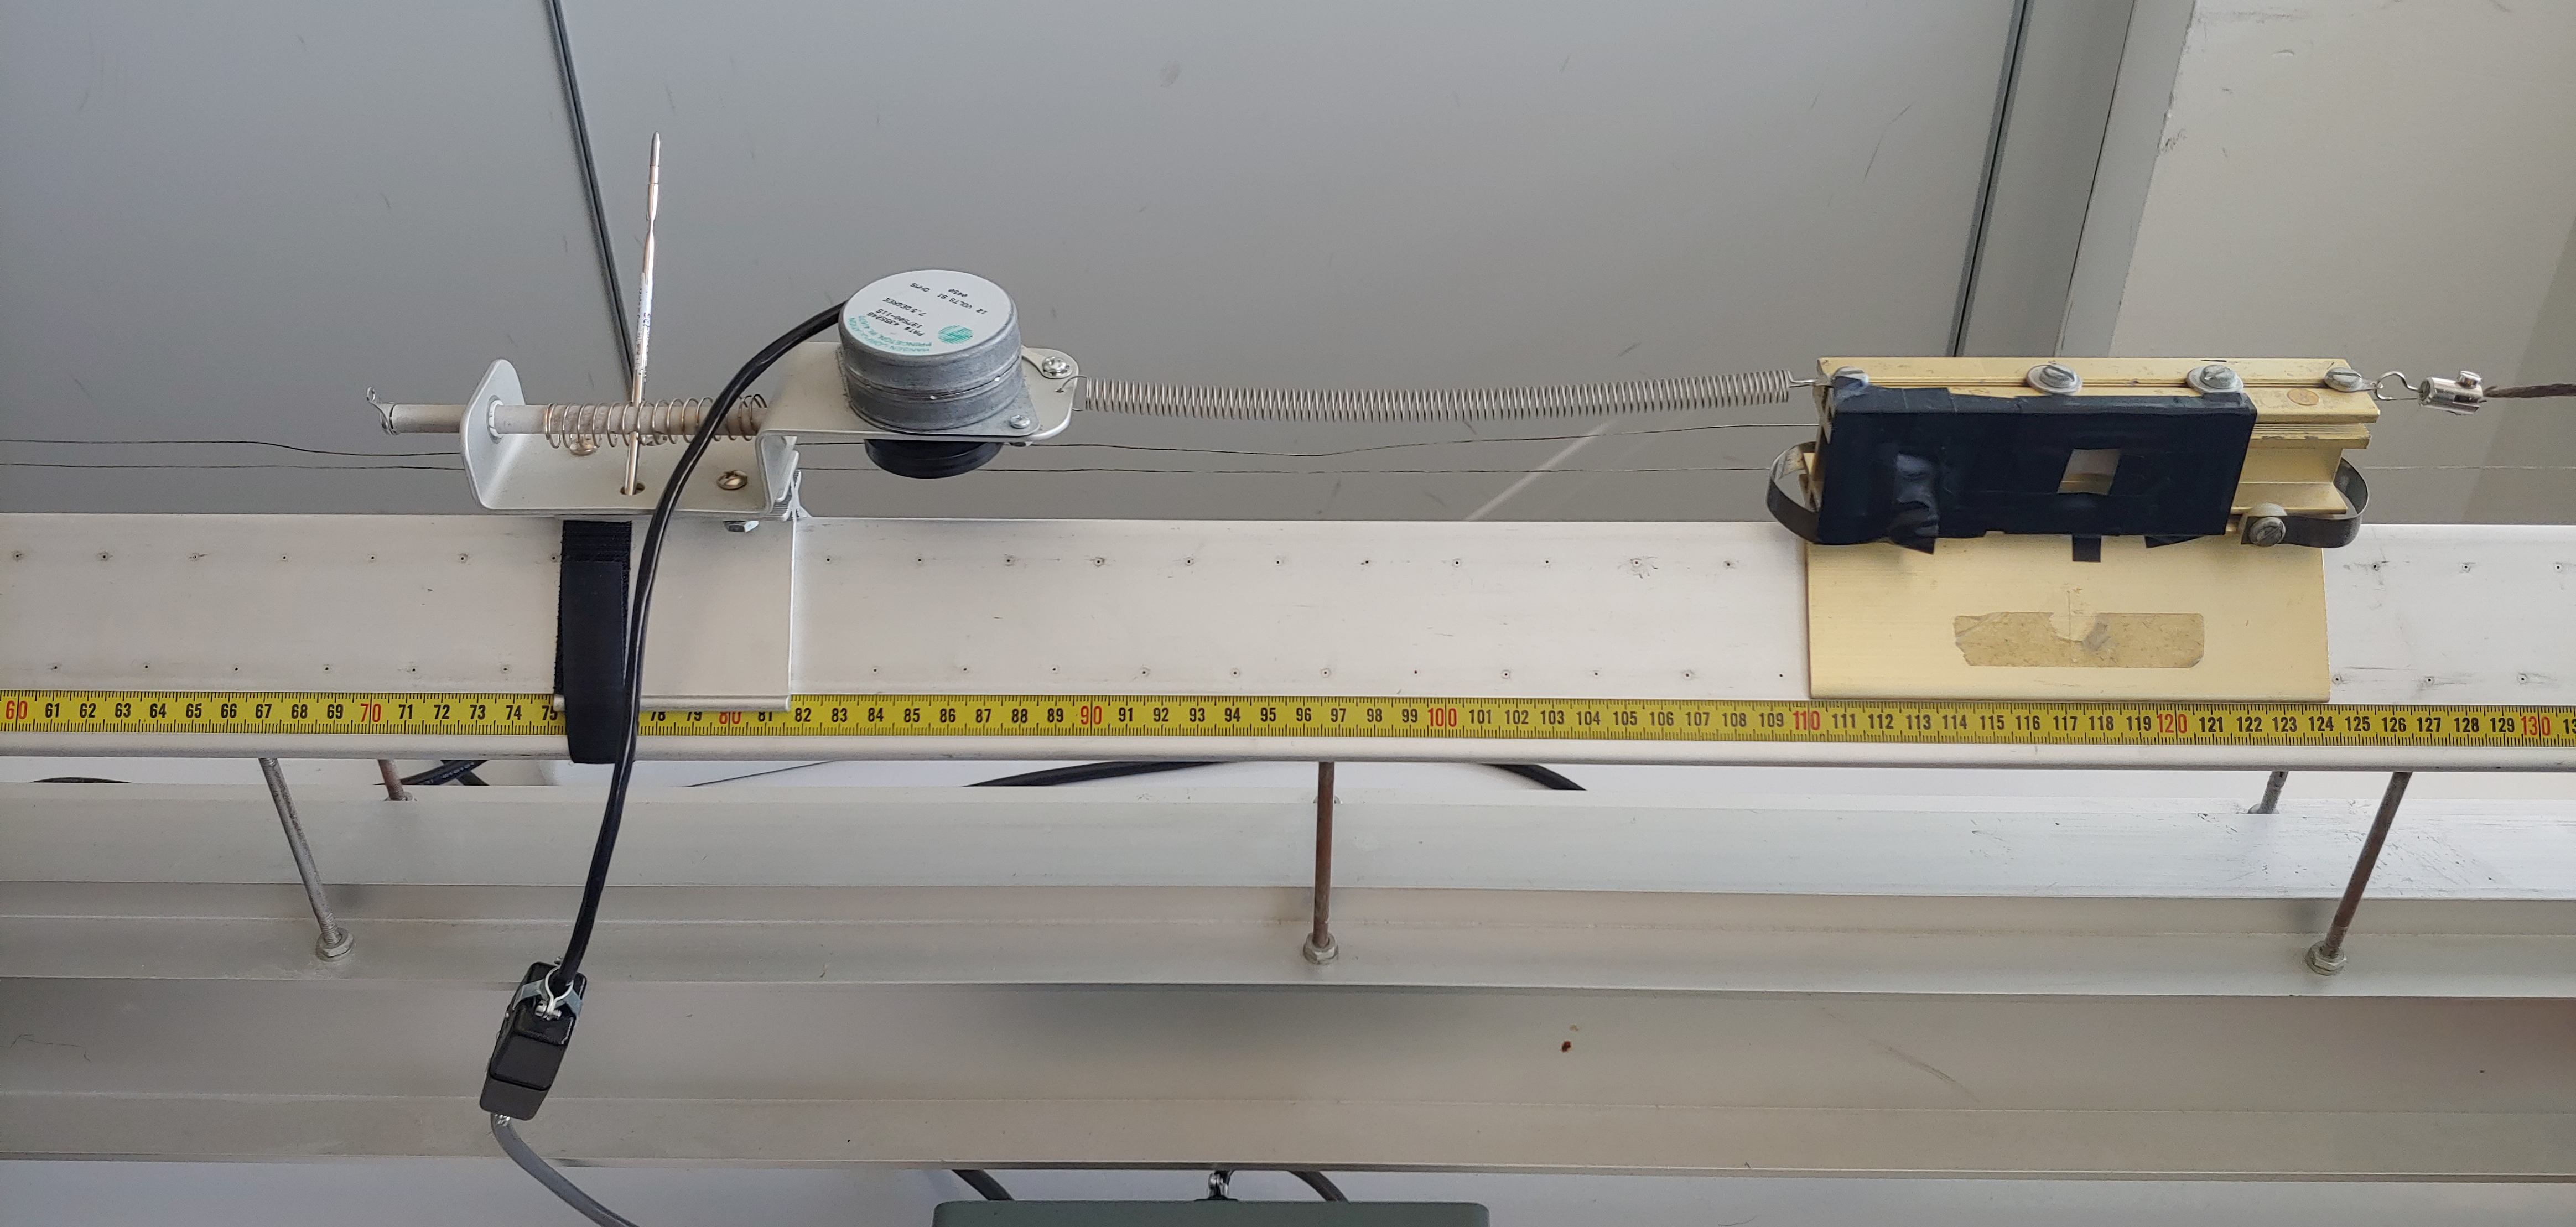
\includegraphics[width=7cm]{fotos/harmonisch.jpg}
              \caption{Foto des Versuchsaufbaus}
          \end{figure}

      \subsection{Messergebnisse}
          Für die Berechnung der Periodendauer haben wir 20 Perioden gemessen vom Zeitpunkt $t_0= 1,1s$ bis $t=12s$\\
          Somit ergibt sich für die Periodendauer:\\
          \begin{equation}
              \begin{gathered}
                  T=\frac{t_{gesamt}}{n}\\
                  T=\frac{12s-1,1s}{20} = 0,545s
              \end{gathered}
          \end{equation}
          Für die Zeit, nach der die Amplitude auf die Hälfte abgenommen hat,  haben wir gemessen: $T_{1/2}=17,5s$\\
          Die maximale Auslenkung beträgt nach Versuchsvorschrift: $x_0=5cm$ \\
          \begin{tikzpicture}
            \begin{axis}[
                    title = {Messwerte: Harmonische Schwingung},
                    xlabel= Zeit \(t\),
                    ylabel= Auslenkung,
                    grid=both,
                    minor grid style={gray!25},
                    major grid style={gray!25},
                    width=0.9\linewidth,
                    height=0.5\linewidth,
                    minor tick num=5,
                ]
                \addplot[line width=0.5pt,solid,color=blue]
                table[x=time,y=position, col sep=comma] {messdaten/harmonisch.csv};
            \end{axis}
        \end{tikzpicture}
      \subsection{Auswertung}
          Bei der Bewegungsgleichung für einen gedämpften harmonischen Oszillator wirkt zusätzlich eine Reibungskraft, die proportional zu der Geschwindigkeit ist,
          \begin{equation}
              F= -b\cdot v\\
          \end{equation}
          mit b die Dämpfungskonstante.
          Das ändert die Lösung der Differentialgleichung.
          Die Bewegungsgleichung lautet dann,
          \begin{equation}
              \ddot{x}+\frac{b}{m}\cdot v+ \frac{k}{m} \cdot x=0
          \end{equation}
          Die Lösung der Differentialgleichung ist die Kombination der e-Funktion mit einer trigonometrischen Formel, da die Amplitude exponentiell abfällt und der Oszillator weiter harmonisch schwingt.
          \begin{equation}
              x(t)= x_0 \cdot e^{ (-b/2m)\cdot t} sin\sqrt{\omega_0^2-\frac{b^2}{4m^2}\cdot t}
          \end{equation}
          Für die Eigenfrequenz ist die Formel so wie bei der ungedämpften Schwingung,
          $\omega_0= \sqrt{\frac{k}{m}}$.\\
          Da es für die Kreisfrequenz auch gilt, $\omega_0=\frac{2\pi}{T}$, ergibt für die Periodendauer (Nährungsweise):
          \begin{equation}\label{periodendauer}
              T=2\pi \sqrt{\frac{m}{k}}
          \end{equation}
          Durch die gemessene Periodendauer kann man die Masse des Gleiters mit der Formel \ref{periodendauer} berechnen, dafür formen wir nach der Masse um:
          \begin{equation}\label{formelm}
              \begin{gathered}
                  T^2=4\pi^2 \frac{m}{k}\\
                  \frac{m}{k}= \frac{T^2}{4\pi^2}\\
                  m= \frac{k\cdot T^2}{4\pi^2}
              \end{gathered}
          \end{equation}
          Da der Gleiter zwischen zwei identischen Federn befestigt ist, muss man darauf achten, dass bei der Federkonstante k(=2k) eingesetzt werden musss.\\
          Also für die Masse des Gleiters ergibt sich:
          \begin{equation}
              m=\frac{2\cdot 21,41 \frac{N}{m} \cdot (0,545s)^2}{4\pi^2}= 0,3222\ kg
          \end{equation}
          Nun berechnen wir die Eigenfrequenz,
          \begin{equation}
              \omega_0= \sqrt{\frac{2\cdot 21,41 \frac{N}{m}}{0,3222kg}} \approx 11,53\ Hz
          \end{equation}
          Die Abklingzeit ist die Zeit, nach der die Amplitude auf 1/e ihres ursprünglichen Werts abgefallen ist, und ist dadurch gegeben,
          \begin{equation}\label{tau}
              \tau = \frac{2m}{b}
          \end{equation}
          Für die Abklingzeit gilt auch:\\
          \begin{equation} \label{abklingszeit}
              \begin{gathered}
                  T_{1/2}= ln(2) \cdot \tau \\
                  T_{1/2}= ln(2) \cdot \frac{2m}{b}
              \end{gathered}
          \end{equation}
          Nun berechnen wir aus Formel \ref{abklingszeit} die Dämpfungskonstante,
          \begin{equation}\label{formelb}
              \begin{gathered}
                  b=\frac{ln(2) \cdot m}{T_{1/2}}\\
                  b= \frac{ln(2) \cdot 0,3222kg}{17,5s} \approx 0,01276 \frac{kg}{s}
              \end{gathered}
          \end{equation}
          Eingesetzt in \ref{tau} ergibt für die Abklingzeit,
          \begin{equation}
              \tau= \frac{2\cdot 0,3222kg}{0,01276\frac{kg}{s}}\approx 50,5s
          \end{equation}
          \subsubsection{Fehlerrechnung}
              Wir berechnen nun die Fehlerfortpflanzung für m nach der Formel:\\
              \begin{equation}\label{fehlerm}
                  \Delta m = \sqrt{\left(\frac{\partial m}{\partial k}\Delta k\right)^2 + \left(\frac{\partial m}{\partial T}\Delta T\right)^2}
              \end{equation}
              Dafür leiten wir die Formel \ref{formelm} nach der einzelnen Variablen ab,\\
              $\frac{\partial m}{\partial k}= \frac{T^2}{4\pi^2}$\\
              $\frac{\partial m}{\partial T}= \frac{kT}{2\pi^2}$\\
              eingesetzt in \ref{fehlerm},
              \begin{equation}
                  \begin{gathered}
                      \Delta m = \sqrt{\left(\frac{T^2}{4\pi^2}\cdot \Delta k\right)^2 + \left(\frac{kT}{2\pi^2}\cdot \Delta T\right)^2}\\
                      \Delta m = \sqrt{\left(\frac{(0,545s)^2}{4\pi^2} \cdot 0,36\frac{N}{m} \right)^2 + \left(\frac{21,41\frac{N}{m}\cdot 0,545s}{2\pi^2} \cdot 0,001s\right)^2}\\
                      \Delta m \approx 0,0028kg=2,8g
                  \end{gathered}
              \end{equation}
              Für die Fehlerfortpflanzung von b leiten wir die Formel  \ref{formelb} nach den einzelnen Variablen ab,\\
              $\frac{\partial b}{\partial m}= \frac{ln(2)}{T_{1/2}}$\\
              $\frac{\partial b}{\partial T_{1/2}}= \frac{-ln(2)\cdot m}{T_{1/2}^2}$\\
              \begin{equation}
                  \begin{gathered}
                      \Delta b = \sqrt{\left(\frac{ln(2)}{T_{1/2}}\cdot \Delta m\right)^2 + \left(\frac{-ln(2)\cdot m}{T_{1/2}^2}\cdot \Delta T_{1/2} \right)^2}\\
                      \Delta b = \sqrt{\left(\frac{ln(2)}{17,5s} \cdot 0,0028kg \right)^2 + \left(\frac{-ln(2)\cdot 0,322kg} {(17,5s)^2}\cdot 0,001s\right)^2}\\
                      \Delta b \approx 0,00011\frac{kg}{s}
                  \end{gathered}
              \end{equation}
          \subsubsection{Endergebnis}
              Insgesamt ergibt sich für m und b:\\
              $m=0,322\pm0,0028kg$\\
              $b= 0,01276\pm 0,00011 \frac{kg}{s}$
      \subsection{Diskussion der Fehler}
          Bei der Messung der Periodendauer und $T_{1/2}$ hat man die CCD-Kamera verwendet, was die Genauigkeit der Messungen sehr deutlich erhöht hat. Somit ergab sich für den Fehler der gerechneten Masse des Gleiters eine Abweichung von 0,87\%. Das ist ein sehr genaues Ergebnis. Die Abweichung bei der Dämpfungskonstante ist auch sehr ähnlich und beträgt 0,86\%. Also die verwendete Methode eignet sich sehr gut für solche Berechnungen. Allerdings ist bei dem Ansatz eine Näherung angenommen wurde, nämlich bei der Berechnung der Periodendauer. Da hat man angenommen, dass T nicht von der Dämpfungskonstante abhängt, was nicht der Realität entspricht. Es hängt davon ab, wie hoch die Dämpfung ist, aber da wir den Versuch mit der Luftkissenbahn durchgeführt haben, könnte man davon ausgehen, dass die Dämpfung schwach ist. Für diesen Fall hätte man für die Periodendauer die Formel: $T=\frac{2\pi}{\sqrt{\omega_0-b^2}}$ verwenden sollen.
          Aber da die Berechnung der Masse damit sehr umständlich wird, konnte man darauf verzichten und die Näherung annehmen.

    \section{Eigenmoden und Schwebung}

      \subsection{Aufbau}
          Wir stellen in diesem Teilversuch nun zwei Gleiter auf die Luftkissenbahn.
          Die Gleiter sind jeweils mit einer Feder (Außenfeder) mit Federkonstante \(k\) am stationären Rand verbunden.
          Miteinander sind sie mit einer Feder (Kopplungsfeder) mit Federkonstante \(k'\) verbunden.

          Wichtig ist das die Kopplungsfeder nicht zu lang ist, da das Sichtfeld der Kamera limitiert ist.
          Wäre sie zu lang, würde der Gleiter aus dem Sichtfeld der Kamera schwingen und es würden keine Werte aufgezeichnet.
          Die CCD-Kamera misst nicht beide Gleiter, sondern in unserem Versuchsaufbau nur die Schwingung des Rechten.

          \begin{figure}[ht]\label{fig:gekoppelt}
              \centering
              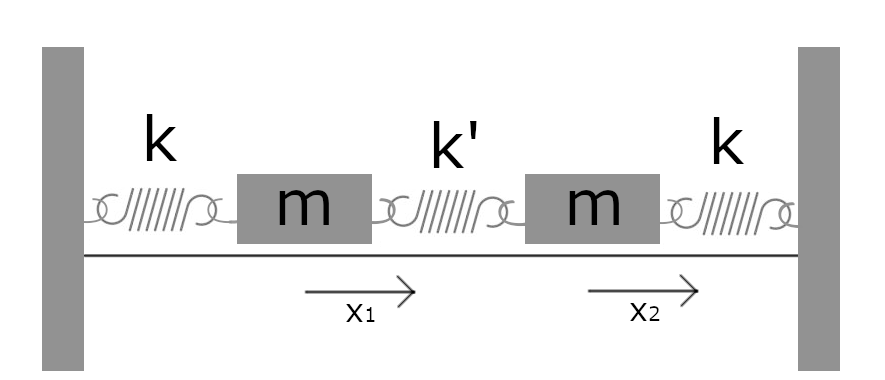
\includegraphics[width=7cm]{fotos/gekoppelt.png}
              \caption{Veranschaulichung des Versuchsaufbau und Bezeichnungen}
          \end{figure}
          (Federbild aus Quelle:\cite{Federn})
          \begin{figure}[ht]\label{fig:foto_schwebung}
              \centering
              \includegraphics[width=7cm]{fotos/schwebung.jpg}
              \caption{Foto des Versuchsaufbaus}
          \end{figure}

      \subsection{Durchführung}
          Die Messaufnahme sollte möglichst vor oder während des Auslenkens bereits gestartet werden.
          Somit ist gewährleistet, das der Anfang der Messungen mit aufgezeichnet wird. Die Messpunkte des Auslenkens stören nicht (Siehe Messergebnisse).
          Diese Durchführung gleicht der des vorherigen Teilversuchs stark.

          Wichtig ist beim Auslenken der Gleiter darauf zu achten, das man nicht zu weit auslenkt, die Amplituden also nicht zu groß werden.
          Die Bewegung wird sonst sehr unkontrolliert, die Federn schlagen auf die Luftkissenbahn und die Gleiter brechen nach oben und zur Seite aus.
          Das ist natürlich nicht förderlich zum akkuraten messen der Schwingungen.
          Für diesen Versuchs ist es auch sinnvoll das Gebläse voll aufzudrehen um die Reibungseffekte klein zu halten, weil wir sie in der Rechnung nicht berücksichtigen

          Wir führen insgesamt drei Messungen durch. Zwei Messungen zu den Eigenmoden und eine für die Schwebung.
          Wir regen in zwei Messungen jeweils eine der beiden Eigenmoden an.
          Zuerst messen wir die gleichphasige Schwingung der beiden Gleiter.
          Dafür werden beide Gleiter um die gleiche Strecke und in die gleiche Richtung aus ihrer Ruhelage ausgelenkt.
          Hierbei sollte möglichst die Kopplungsfeder, die die beiden Gleiter verbindet nicht gestreckt oder gestaucht werden.
          Die Kopplungsfeder ist eigentlich nicht Teil dieser Eigenschwingung,
          es ist in der experimentellen Durchführung aber fast unmöglich das sie wirklich inaktiv bleibt.

          Als zweites messen wir die gegenphasige Schwingung.
          Hierbei lenken wir beide Gleiter in entgegengesetzte Richtungen aus. Bewegen sie also aufeinander zu.
          Für diese Messungen achtet man verstärkt darauf, dass die Gleiter den gleichen Abstand zum Rand haben,
          um sicher zugehen, dass man sie wirklich um die gleiche Strecke ausgelenkt hat.

          Als letztes messen wir noch die Schwebung.
          Dazu wird der rechte Gleiter in seiner Ruhelage festgehalten und der linke Gleiter nach zum ihm näher liegenden Rand ausgelenkt.
          Die beiden Gleiter verhalten sich hier nicht gleich oder spiegelverkehrt wie in den vorherigen beiden Messungen,
          deshalb ist es wichtig zu wissen welche der Bewegungen der Gleiter wir aufzeichnen.
          Wir haben den rechten, zunächst stationären Gleiter gemessen.

      \subsection{Messergebnisse}
          \subsubsection{Messwerte für die beiden Eigenmoden}
              \begin{tikzpicture}
                  \begin{axis}[
                          title = {Messwerte: Gleichphasige Schwingung},
                          xlabel=Zeit \(t\) in Sekunden,
                          ylabel=Amplitude,
                          grid=both,
                          minor grid style={gray!25},
                          major grid style={gray!25},
                          width=0.45\linewidth,
                          minor tick num=5,
                      ]
                      \addplot[line width=0.5pt,solid,color=blue]
                      table[x=time,y=position, col sep=comma] {messdaten/gleich_phasig.csv};

                      \addplot[mark=*,black] plot coordinates {
                              (9.9,2034)
                              (34.2,1758)
                          };
                  \end{axis}
              \end{tikzpicture} %
              \begin{tikzpicture}
                  \begin{axis}[
                          title = {Messwerte: Gegenphasige Schwingung},
                          xlabel=Zeit \(t\) in Sekunden,
                          ylabel=Amplitude,
                          grid=both,
                          minor grid style={gray!25},
                          major grid style={gray!25},
                          width=0.45\linewidth,
                          minor tick num=5,
                      ]
                      \addplot[line width=0.5pt,solid,color=blue]
                      table[x=time,y=position, col sep=comma] {messdaten/gegen_phasig.csv};

                      \addplot[mark=*,black] plot coordinates {
                              (3.3,1901)
                              (23.7,1630)
                          };
                  \end{axis}
              \end{tikzpicture}\\
              Die Amplitudeneinheiten sind hier willkürlich vom Messprogramm. Sie sind einheitenlos und spielen für die Auswertung dieses Versuchs keine Rolle. \\
              Man sieht bei beiden Messungen am Anfang noch einen Teil des manuellen Auslenkens.

              Aus diesen beiden Messungen haben wir die Schwingungsdauern bestimmt, indem wir Werte aus den Diagrammen ausgelesen haben.
              Wir haben dafür mehrere Perioden (\(n\) Stück) gezählt und die verstrichene Zeit zwischen den Maxima berechnet.
              Durch diesen Durchschnitt haben wir versucht den Messfehler klein zuhalten.
              Die abgelesenen Werte sind in den Diagrammen markiert.

              Für die Schwingungsdauer \(T_{-}\) (gleichphasige Schwingung) haben wir die folgenden Werte gemessen:
              \begin{figure}[ht]
                  \centering
                  \begin{tabular}{|c | c | c|}
                      \hline
                      Zeit des ersten Maximum \(t_0\) & Zeit des letzten Maximum \(t_1\) & Periodenanzahl \(n\) \\
                      \hline
                      \SI{9.9}{\second}               & \SI{34.2}{\second}               & 30 \\
                      \hline
                  \end{tabular}
              \end{figure}

              Für die Schwingungsdauer \(T_{+}\) (gegenphasige Schwingung) haben wir die folgenden Werte gemessen:
              \begin{figure}[ht]
                  \centering
                  \begin{tabular}{|c | c | c|}
                      \hline
                      Zeit des ersten Maximum \(t_0\) & Zeit des letzten Maximum \(t_1\) & Periodenanzahl \(n\) \\
                      \hline
                      \SI{3.3}{\second}               & \SI{23.7}{\second}               & 30 \\
                      \hline
                  \end{tabular}
              \end{figure}

          \subsubsection{Messwerte für die Schwebung}
              \begin{center}\label{fig:messung_schwebung}
                  \begin{tikzpicture}
                      \begin{axis}[
                              title = {Messwerte: Schwebung},
                              xlabel=Zeit \(t\) in Sekunden,
                              ylabel=Amplitude,
                              grid=both,
                              minor grid style={gray!25},
                              major grid style={gray!25},
                              width=0.9\linewidth,
                              height=0.5\linewidth,
                              minor tick num=5,
                          ]
                          \addplot[line width=0.5pt,solid,color=blue]
                          table[x=time,y=position, col sep=comma,] {messdaten/schwebung.csv};

                          \addplot[mark=*,black] plot coordinates {
                                  (1.8,1913)
                                  (25.6,1685)
                              };
                          \addplot[mark=*,red] plot coordinates {
                                  (4.2,1339)
                                  (53.0,1329)
                              };
                      \end{axis}
                  \end{tikzpicture}
              \end{center}

              Für die Schwingungsdauer \(T_{\omega_0}\) (Schwingungsfrequenz der Gleiter) haben wir die folgenden Werte gemessen:
              \begin{figure}[ht]
                  \centering
                  \begin{tabular}{|c | c | c|}
                      \hline
                      Zeit beim des Maximum \(t_0\) & Zeit des letzten Maximum \(t_1\) & Periodenanzahl \(n\) \\
                      \hline
                      \SI{1.8}{\second}             & \SI{25.6}{\second}               & 30 \\
                      \hline
                  \end{tabular}
              \end{figure}

              Für die Schwingungsdauer \(T_{\Delta \omega}\) (Schwebungsfrequenz) haben wir die folgenden Werte gemessen:
              \begin{figure}[ht]
                  \centering
                  \begin{tabular}{|c | c | c|}
                      \hline
                      Zeit des ersten Minimums \(t_0\) & Zeit des letzten Minimums \(t_1\) & Periodenanzahl \(n\) \\
                      \hline
                      \SI{4.2}{\second}                & \SI{53}{\second}                  & 5 \\
                      \hline
                  \end{tabular}
              \end{figure}

      \subsection{Auswertung}
          \subsubsection{Theorie und Formeln}
              Wir wollen unsere gemessenen Periodendauern (und Kreisfrequenzen) mit den theoretischen Werten vergleichen.
              Diese theoretischen Werte können wir aus der in den vorherigen Versuchen bestimmten Masse \( m \) der Gleiter und den Federkonstante
              der beiden Federn \( k \) und \( k' \) bestimmen.

              \paragraph{Eigenmoden}
                  Wir betrachten zunächst die beiden Eigenmoden des Systems.
                  Das \enquote{schwingfähige System} sind die beiden schwingenden Gleiter mit den drei Federn.
                  Eine Eigenmode oder Normalmode ist eine spezielle Bewegung eines schwingfähigen Systems.
                  Bei diesen Bewegungen haben alle Komponenten des Systems die gleiche Frequenz. Die Gleiter schwingen dann also mit der gleichen Frequenz.
                  Mit den beiden Eigenmoden können alle theoretisch möglichen Bewegungen des Systems dargestellt werden (Vergleiche Eigenbasis, Eigenwert).
                  Durch Kombination der beiden Eigenmoden, können wir dann später die komplexe Bewegung der Schwebung beschreiben. (Aus:~\cite{Eigenmode})

                  Für die nachfolgende Berechnung betrachten wir die Reibung des Systems nicht.
                  Sie ist, wie wir im vorherigen Versuch gezeigt und berechnet haben durchaus existent.
                  Der Reibungskoeffizient würde in den Schwingungsfrequenzen der beiden Eigenmoden auftauchen, würde also das hier berechnete Ergebnis verändern.
                  Unser schwingfähiges System besteht aus zwei beweglichen Teilen, den beiden Gleitern auf der Luftkissenbahn,
                  wegen dieser zwei Freiheitsgrade hat das System auch zwei Eigenmoden.
                  Im Experiment haben wir diese beiden Eigenschwingungen angeregt, wir berechnen hier zum theoretischen Vergleich zunächst die beiden Eigenfrequenzen.

                  Die erste der beiden Eigenmoden ist die gleichphasige Bewegung der beiden Gleiter.
                  Sie schwingen dann mit konstantem Abstand zu einander und haben dadurch keine Phasendifferenz.
                  Die Kopplungsfeder \(k'\) übt dabei, da der Abstand zwischen den beiden Gleitern gleicht bleibt, während der Schwingung keine Kräfte aus.
                  Sie muss also beim Start des Experiments möglichst ungespannt sein.

                  Die Frequenz dieser Eigenschwingung ist, da wegen der inaktiven Kopplungsfeder auf einen Gleiter immer nur die Feder wirkt, die ihn mit dem Rand verbindet gleich der Frequenz des ungekoppelten Pendels.
                  Sie ist aber nicht gleich zum vorherigen Versuchsteil, weil wir im Versuch davor zwei Federn mit Federkonstante \(k\) benutzt haben, auf beiden Seiten eines Gleiters.
                  Hier schwingen nun zwei Gleiter jeder aber nur mit einer Feder mit Federkonstante \(k\).

                  Da bei einer Eigenmode, wie oben beschrieben alle Komponenten, hier die Gleiter, die gleiche Frequenz haben, reicht es sich die Kräfte auf
                  einen Gleiter anzuschauen und seine Schwingungsfrequenz zu bestimmen.
                  Auf den linken Gleiter wirkt, da die mittlere Feder nicht an ihm zieht, nur die Federkraft der äußeren Feder.
                  Sie wirkt hier in negative \(x_1\)-Richtung (Siehe~\ref{fig:gekoppelt}). Es gilt also:
                  \begin{equation}
                      F = -k \cdot x
                  \end{equation}
                  Wir setzen die für die Kraft die Trägheit des Gleiters ein. Die Beschleunigung ist die zweite Ableitung des Ortes, wir ersetzen also \( a = \ddot{x} \):
                  \begin{equation}
                      \begin{gathered}
                          m \cdot a = -k \cdot x \\
                          \Rightarrow m \cdot \ddot{x} = -k \cdot x
                      \end{gathered}
                  \end{equation}
                  Die Lösung dieser Differenzialgleichung zweiter Ordnung ist eine Sinusfunktion der Form:
                  \begin{equation}
                      \begin{aligned}\label{eq:ansatz}
                          x(t) =        & A \cdot \sin( \omega \cdot t + \varphi )                 \\
                          \ddot{x}(t) = & -A \cdot \omega^2 \cdot \sin( \omega \cdot t + \varphi )
                      \end{aligned}
                  \end{equation}
                  Setzen wir die Lösung und ihre zweite Ableitung in die Differenzialgleichung ein erhalten wir:
                  \begin{equation}
                      \begin{gathered}
                          m \cdot \cancel{-A} \cdot \omega^2 \cdot \cancel{\sin( \omega \cdot t + \varphi)} = \cancel{-}k \cdot \cancel{A} \cdot \cancel{\sin( \omega \cdot t + \varphi )} \\
                          \Rightarrow m \cdot \omega^2 = k \\
                          \Rightarrow \omega^2 = \frac{k}{m} \\
                      \end{gathered}
                  \end{equation}
                  Ziehen wir noch die Wurzel erhalten wir die Eigenfrequenz für die gleichphasige Schwingung \(\omega_{-}\).
                  \begin{equation}\label{eq:omega_minus}
                      \omega_{-} = \sqrt{ \frac{k}{m} }
                  \end{equation}

                  Für die gegenphasige Schwingung führen die Gleiter eine gegenläufige Schwingungen aus.
                  Die Gleiter schwingen demnach mit einer Phasendifferenz von \( \pi \).
                  Die rücktreibenden Kräfte stammen jeweils aus der Deformation der Außenfeder \(k\), sowie der Kopplungsfeder \(k'\).
                  Da aber beide Gleiter, sowohl der Linke, als auch der Rechte, schwingen und beide auf die Kopplungsfeder drücken, wird die Feder von beide gestaucht (oder verlängert).
                  Ihre Längenänderung ist also zweimal so groß wie diejenige der Federn \(k\), da auf die Außenfedern immer nur ein Gleiter drückt.
                  Die resultierende Federkraft ist damit für die Stauchung \(x\) durch das Hookesche Gesetz doppelt so groß \( F_{\text{Kopplungsfeder}} = 2 k' \cdot x \), wie wenn nur ein Gleiter schwingen würde.

                  Wir stellen erneut die Kräftegleichung auf; wir betrachten wieder den linken Gleiter.
                  Die Außenfeder zieht hier wieder in negative \(x_1\)-Richtung. Die Kopplungsfeder drückt in die gleiche Richtung.
                  \begin{equation}
                      \begin{aligned}
                          F & = -k \cdot x - 2 k' \cdot x \\
                            & = -x \cdot ( k + 2 k')
                      \end{aligned}
                  \end{equation}
                  Wie oben ersetzen wir wieder die Beschleunigung durch die zweite Ableitung des Ortes:
                  \begin{equation}
                      \begin{aligned}
                          m \cdot a                    & = -x \cdot ( k + 2 k') \\
                          \Rightarrow m \cdot \ddot{x} & = -x \cdot ( k + 2k')
                      \end{aligned}
                  \end{equation}
                  Auch hier löst der trigonometrische Ansatz aus Gleichung~(\ref{eq:ansatz}) die Differenzialgleichung. Setzen wir ihn ein erhalten wir:
                  \begin{equation}
                      \begin{aligned}
                          m \cdot \left( \cancel{-A} \cdot \omega^2 \cdot \cancel{ \sin( \omega \cdot t + \varphi ) } \right) & = \cancel{-A} \cdot \cancel{\sin( \omega \cdot t + \varphi )} \cdot ( k + 2 k' ) \\
                          \Rightarrow m \cdot \omega^2                                                                        & = (k + 2 k')                                                                     \\
                          \Rightarrow \omega^2                                                                                & = \frac{ k + 2k' }{ m }
                      \end{aligned}
                  \end{equation}
                  Ziehen wir hier die Wurzel erhalten wir die Eigenfrequenz für die gegenphasige Schwingung \( \omega_{+} \).
                  \begin{equation}\label{eq:omega_plus}
                      \omega_{+} = \sqrt{ \frac{ k + 2 k' }{m} }
                  \end{equation}
                  Da hier über dem Bruch die zusätzlich die Federkonstante der Kopplungsfeder steht (Vergleiche:~\ref{eq:omega_minus}) ist die Eigenfrequenz der gegenphasigen Schwingung
                  immer größer als die Eigenfrequenz der Gleichphasigen. Unabhängig, von den gewählten Masse der Gleiter, sowie der gewählten Federn.\label{Plus_größer_Minus}

              \paragraph{Schwebung}
                  Wir setzen nun die beiden Eigenfrequenzen wieder in den Ansatz~(\ref{eq:ansatz}) ein.
                  Die beiden Funktionen sind hier in allgemeiner Form, dass heißt es wurden noch keine Anfangsbedingungen eingesetzt.
                  \begin{equation}
                      \begin{gathered}
                          x_{+}(t) = A \cdot \sin( \omega_{+} \cdot t + \varphi_{+} ) \\
                          x_{-}(t) = A \cdot \sin( \omega_{-} \cdot t + \varphi_{-} ) \\
                      \end{gathered}
                  \end{equation}
                  Wir wollen nun die Bewegungsgleichungen der beiden Gleiter im Fall der Schwebung aufstellen.
                  Wie oben bereits erklärt lässt sich dieser Zustand als Kombination der beiden Eigenmoden beschreiben.
                  Wir addieren/subtrahieren, also die beiden Eigenschwingungen. (Ansatz aus der Vorlesung:~Addition zweier Schwingungen~\cite{ExPhy1}).
                  Hierfür verwenden wir die Additionstheoreme von Sinus und Kosinus (Summen zweier trigonometrischer Funktionen~\cite{Trigonometrie}). \\
                  Einmal addieren:
                  \begin{equation}
                      \begin{gathered}\label{eq:x1_umformung}
                          x_1(t) = x_{+}(t) + x_{-}(t) = A \cdot ( \sin( \omega_{+} \cdot t + \varphi_{+} ) + \sin( \omega_{-} \cdot t + \varphi_{-} ) ) \\
                          = A \cdot \left( 2 \cdot \sin\left( \frac{ \omega_{+} \cdot t + \varphi_{+} + \omega_{-} \cdot t + \varphi_{-} }{2} \right) \cdot \cos\left( \frac{ \omega_{+} \cdot t + \varphi_{+} - \left( \omega_{-} \cdot t + \varphi_{-} \right) }{2} \right) \right)
                      \end{gathered}
                  \end{equation}
                  Und einmal subtrahieren:
                  \begin{equation}\label{eq:x2_umformung}
                      \begin{gathered}
                          x_2(t) = x_{+}(t) - x_{-}(t)
                          = A \cdot ( \sin( \omega_{+} \cdot t + \varphi_{+} ) - \sin( \omega_{-} \cdot t + \varphi_{-} ) ) \\
                          = A \cdot \left( 2 \cdot \cos\left( \frac{ \omega_{+} \cdot t + \varphi_{+} + \omega_{-} \cdot t + \varphi_{-} }{2} \right) \cdot \sin\left( \frac{ \omega_{+} \cdot t + \varphi_{+} - \left( \omega_{-} \cdot t + \varphi_{-} \right) }{2} \right) \right)
                      \end{gathered}
                  \end{equation}

                  Wir führen hier jetzt zwei neue Frequenzen ein. Sie beschreiben die bei der Schwebung auftretenden Frequenzen.
                  Beide Gleiter schwingen mit der Frequenz \(\omega_0\) um ihren Nullpunkt.
                  Die Amplitude dieser Schwingung ändert sich (phasenverschoben um \( \frac{\pi}{2} \)) mit der wesentlich kleineren Frequenz \( \Delta \omega \).
                  Diese langsame Amplitudenschwingung bezeichnet man auch als \enquote{Einhüllende}.

                  Zwischen den beiden neu eingeführten Frequenzen und den beiden Eigenfrequenzen des System besteht der nachfolgende Zusammenhang.
                  \begin{equation}\label{eq:omega_null}
                      \omega_0 = \frac{ \omega_{+} + \omega{-} }{ 2 }
                  \end{equation}
                  \begin{equation}\label{eq:delta_omega}
                      \Delta \omega = \frac{ \omega_{+} - \omega{-} }{ 2 }
                  \end{equation}
                  Setzen wir die beiden Beziehungen ein vereinfachen sich unsere Funktionen zu:
                  \begin{equation}
                      \begin{gathered}
                          x_1(t) = 2 \cdot A \cdot \left( \sin\left( \omega_0 \cdot t + \frac{\varphi_{+} + \varphi_{-} }{2} \right) \cdot \cos\left( \Delta \omega \cdot t + \frac{\varphi_{+} - \varphi_{-} }{2} \right) \right) \\
                          x_2(t) = 2 \cdot A \cdot \left( \cos\left( \omega_0 \cdot t + \frac{\varphi_{+} + \varphi_{-} }{2} \right) \cdot \sin\left( \Delta \omega \cdot t + \frac{\varphi_{+} - \varphi_{-} }{2} \right) \right)
                      \end{gathered}
                  \end{equation}
                  Bei diesen beiden Funktionen handelt es sich um die allgemeine Lösungen des schwingenden Systems.
                  Das heißt man kann mit ihnen, egal wie man die Gleiter auslenkt oder anstößt, das System beschreiben.

                  Wir haben bei unserer experimentellen Durchführung den linken Gleiter aus seiner Ruhelage ausgelenkt und den Rechten festgehalten.
                  Die beiden Gleiter hatten damit zum Zeitpunkt \(t = 0\) also keine Geschwindigkeit \( v(0) = 0\).

                  Die beiden Gleiter schwingen, wie in der Abbildung~(\ref{fig:gekoppelt}) angedeutet, um ihren jeweiligen Nullpunkt.
                  Da wir den linken Gleiter auslenken ist er zum Zeitpunkt \(t = 0\) am Ort (gemessen mit \(x_1\)-Achse) \(x_1(0) = -2 \cdot A \).
                  Der rechte Gleiter wird nicht ausgelenkt ist also zum Zeitpunkt \(t = 0\) am Ort (gemessen mit \(x_2\)-Achse) \(x_2(0) = 0\)

                  Mit diesen Anfangsbedingungen bestimmen wir jetzt die spezielle Lösung des Systems.
                  Setzen wir die Anfangsbedingung für die Startauslenkung für \(x_1(t)\) ein (Nicht umgeformt, Vergleiche~(\ref{eq:x1_umformung})), so erhalten wir:
                  \begin{equation}
                      x_1(0) = - 2 \cdot A = A \cdot \sin \left( \varphi_{+} \right) + A \cdot \sin \left( \varphi_{-} \right)
                  \end{equation}
                  \(\varphi_{+}\) und \( \varphi_{-} \) müssen also \(-\frac{\pi}{2}\) sein.

                  Wir überprüfen noch, dass dieser Wert für \(\varphi_{+}\), \( \varphi_{-} \) auch die Bedingung erfüllt, dass die Anfangsgeschwindigkeit gleich Null ist.
                  Dafür leiten wir die Funktion \(x_1(t)\) nach der Zeit ab. Wir erhalten die zeitabhängige Geschwindigkeit:
                  \begin{equation}
                      \begin{gathered}
                          v_1(t) = \frac{\mathrm{d}}{\mathrm{d} t} x_1(t) = 2 \cdot A \cdot \bigg(
                          \omega_0 \cdot \cos \left( \omega_0 \cdot t + \frac{\varphi_{+} + \varphi_{-} }{2} \right) \cdot \cos\left( \Delta \omega \cdot t + \frac{\varphi_{+} - \varphi_{-} }{2} \right) \\
                          - \Delta \omega \cdot \sin\left( \omega_0 \cdot t + \frac{\varphi_{+} + \varphi_{-} }{2} \right) \cdot \sin\left( \Delta \omega \cdot t + \frac{\varphi_{+} - \varphi_{-} }{2} \right) \bigg) \\
                      \end{gathered}
                  \end{equation}
                  Setzen wir hier \(t = 0\) und \(v(0) = 0\) ein, so erhalten wir:
                  \begin{equation}
                      v_1(0) = 0 = \omega_0 \cos \left( \frac{\varphi_{+} + \varphi_{-} }{2} \right) \cdot \cos \left( \frac{\varphi_{+} - \varphi_{-} }{2} \right) - \Delta \omega \sin \left( \frac{\varphi_{+} + \varphi_{-} }{2} \right) \cdot \sin \left( \frac{\varphi_{+} - \varphi_{-} }{2} \right)
                  \end{equation}
                  Wir setzen hier weiter \( \frac{-\pi}{2} \) für die beiden Phasen ein:
                  \begin{equation}
                      \begin{gathered}
                          v_1(0) = 0 = \omega_0 \cos \left( \frac{ \frac{-\pi}{2} + \frac{-\pi}{2} }{2} \right) \cdot \cos \left( \frac{ \frac{-\pi}{2} - \frac{-\pi}{2} }{2} \right) - \Delta \omega \sin \left( \frac{ \frac{-\pi}{2} + \frac{-\pi}{2} }{2} \right) \cdot \sin \left( \frac{ \frac{-\pi}{2} - \frac{-\pi}{2} }{2} \right) \\
                          = \omega_0 \cos \left( \frac{-\pi}{2} \right) \cdot \cos \left( 0 \right) - \Delta \omega \sin \left( \frac{-\pi}{2} \right) \cdot \sin \left( 0 \right) \\
                          = \omega_0 \cdot 0 \cdot 1 - \Delta \omega \cdot 1 \cdot 0 = 0
                      \end{gathered}
                  \end{equation}
                  Die bestimmten Werte erfüllen, also auch die zweite Bedingung.

                  Nun weiter für die Funktion \(x_2(t)\):
                  Für den zweiten Gleiter muss die Amplitude am Anfang Null betragen, also \( x_2(0) = 0\). (Wie oben nicht umgeformt, Vergleiche~(\ref{eq:x2_umformung}))
                  \begin{equation}
                      x_2(0) = 0 = A \cdot \sin \left( \varphi_{+} \right) - A \cdot \sin \left( \varphi_{-} \right)
                  \end{equation}
                  Die beiden Phasen müssen also gleich sein. Wir definieren \(\varphi := \varphi_{+} = \varphi_{-}\).

                  Weiterhin betrachten wir die Geschwindigkeitsbedingung.
                  Die Geschwindigkeitsfunktion \(v_2(t)\) ist bis auf vertauschte \( \omega_0 \) und \( \Delta \omega \), die Selbe wie für \( x_1(t) \).
                  Wir setzen erneut \(t = 0\) und \( v_2(0) = 0 \) ein, sowie unsere neue Bedingung \( \varphi_{+} = \varphi_{-} \) und erhalten:
                  \begin{equation}
                      \begin{aligned}
                          v_2(0) = 0 & = \Delta \omega \cos \left( \frac{\varphi + \varphi }{2} \right) \cdot \cos \left( \frac{\varphi - \varphi }{2} \right) - \omega_0 \sin \left( \frac{\varphi + \varphi }{2} \right) \cdot \sin \left( \frac{\varphi - \varphi }{2} \right) \\
                                     & = \Delta \omega \cos \left( \frac{\varphi + \varphi }{2} \right) \cdot \cos \left( 0 \right) - \omega_0 \sin \left( \frac{\varphi + \varphi }{2} \right) \cdot \sin \left( 0 \right)                                                       \\
                                     & = \Delta \omega \cos \left( \frac{\varphi + \varphi }{2} \right) - 0
                      \end{aligned}
                  \end{equation}
                  Damit die Bedingung erfüllt ist muss der Kosinus Null sein. Sein Argument, damit also \( \frac{\pi}{2}\) oder \( \frac{\pi}{2}\) plus ein ganzzahliges Vielfaches von \(\pi\).
                  Diese Lösungen sind alle äquivalent, da sie die Funktion nur verschieben. Wir wählen \( \frac{\pi}{2} \).
                  \begin{equation}
                      \frac{ \varphi + \varphi }{ 2 } = \frac{\pi}{2}
                  \end{equation}
                  Also ist \(\varphi = \frac{\pi}{2} \)

                  Setzen wir die bestimmte Anfangsbedingungen für die erste Funktion ein erhalten wir:
                  \begin{equation} % TODO: Minus
                      \begin{gathered}
                          x_1(t) = 2 \cdot A \cdot \sin \left( \omega_0 \cdot t + \frac{ \frac{-\pi}{2} + \frac{-\pi}{2}}{2} \right) \cdot \cos \left( \Delta \omega \cdot t + \frac{ \frac{- \pi}{2} - \frac{- \pi}{2} }{2} \right) \\
                          = 2 \cdot A \cdot \sin \left( \omega_0 \cdot t - \frac{\pi}{2} \right) \cdot \cos \left( \Delta \omega \cdot t \right) \\
                          = 2 \cdot A \cdot \cos \left( \omega_0 \cdot t \right) \cdot \cos \left( \Delta \omega \cdot t \right)
                      \end{gathered}
                  \end{equation} % TODO: Minus
                  Und für die zweite Funktion:
                  \begin{equation}
                      \begin{gathered}
                          x_2(t) = 2 \cdot A \cdot \cos\left( \omega_0 \cdot t + \frac{ \frac{\pi}{2} + \frac{\pi}{2} }{2} \right) \cdot \sin\left( \Delta \omega \cdot t + \frac{ \frac{\pi}{2} - \frac{\pi}{2} }{2} \right) \\
                          = 2 \cdot A \cdot \cos\left( \omega_0 \cdot t + \frac{\pi}{2} \right) \cdot \sin\left( \Delta \omega \cdot t \right) \\
                          = 2 \cdot A \cdot \sin \left( \omega_0 \cdot t \right) \cdot \sin\left( \Delta \omega \cdot t \right)
                      \end{gathered}
                  \end{equation}
                  Die beiden Funktionen lauten also:
                  \begin{equation}
                      \begin{gathered}\label{eq:bewegungsfunktionen}
                          \text{Pendel 1: } x_1(t) = 2 A \cos( \Delta \omega t ) \cdot \cos( \omega_0 t) \\
                          \text{Pendel 2: } x_2(t) = 2 A \sin( \Delta \omega t ) \cdot \sin( \omega_0 t)
                      \end{gathered}
                  \end{equation}
                  Hierbei ist \(x_1(t)\) die Auslenkung des linken Gleiters und \(x_2(t)\) die Auslenkung des rechten Gleiters, jeweils aus der dazugehörigen Ruhelage. \\

                  Wir veranschaulichen uns diese beiden Lösungsfunktionen noch einmal.
                  Für beispielhafte, zu unseren Gegebenheiten passenden Werte, ergeben sich die folgenden beiden Graphen: \\
                  \begin{tikzpicture} % Omega Null = 10, Delta Omega = 1, Amplitude = 1
                      \begin{axis}[
                              title = {Veranschaulichung der Lösungsfunktionen \(x_1\)},
                              xlabel= Zeit \(t\),
                              ylabel= Auslenkung,
                              grid=both,
                              minor grid style={gray!25},
                              major grid style={gray!25},
                              width=0.45\linewidth,
                              minor tick num=5,
                          ]
                          \addplot[
                              domain=0:15,
                              samples=1000,
                              line width=1pt,
                              solid,
                              color=blue] {2 * 1 * cos(1 * deg(x)) * cos(10 * deg(x)) };
                      \end{axis}
                  \end{tikzpicture} %
                  \begin{tikzpicture} % Omega Null = 10, Delta Omega = 1, Amplitude = 1
                      \begin{axis}[
                              title = {Veranschaulichung der Lösungsfunktionen \(x_2\)},
                              xlabel= Zeit \(t\),
                              ylabel= Auslenkung,
                              grid=both,
                              minor grid style={gray!25},
                              major grid style={gray!25},
                              width=0.45\linewidth,
                              minor tick num=5,
                          ]
                          \addplot[
                              domain=0:15,
                              samples=1000,
                              line width=1pt,
                              solid,
                              color=blue] {2 * 1 * sin(1 * deg(x)) * sin( 10 * deg(x)) };
                      \end{axis}
                  \end{tikzpicture}\\
                  Aus den Graphen können wir unsere Anfangswerte ablesen. Wir sehen im linken Graphen, das der Gleiter bei maximaler Auslenkung startet, im Rechten, das er bei Null startet.
                  Wir haben also richtig gerechnet, da sich unsere Anfangsbedingungen hier wieder spiegeln.

                  Wir können hier die beiden theoretischen Funktionen auch gut mit den echten Messwerte vergleichen.
                  Gemessen wurde der rechte Gleiter, darum starten die Messwerte auch bei Null. (Vergleiche:~\ref{fig:messung_schwebung})

                  Hier kann man sehr gut erkennen, warum wir die beiden neuen Frequenzen eingeführt haben.
                  Die schnelle Frequenz \(\omega_0\) ist die Frequenz mit der die Gleiter schwingen. Die entsprechende Schwingungsdauer also die Zeit zwischen den Maxima.
                  Die langsame Frequenz \(\Delta \omega \) ist die Frequenz mit der sich die Amplitude ändert. Sie erkennt man hier an der einhüllenden Sinusschwingung.
                  Also die Kurve um die kleinen kugelförmigen \enquote{Päckchen}.

                  Auch etwas Physik können wir hier ablesen.
                  Der nicht ausgelenkte Gleiter wird zum Start des Experiments zunächst von der Kopplungsfeder in Richtung der ausgelenkten Feder gezogen (Erstes Maximum im linken Graphen).
                  Da der linke Gleiter aber in seine Ruhelage zurückkehrt, wird der rechte Gleiter wieder über seine Ruhelage hinaus gedrückt.
                  Er wird weil nun die linke Außenfeder und die Kopplungsfeder ihn nach links drücken bereits ein gutes Stück nach rechts.

                  (Quelle: Gekoppelte Pendel~2.1.2.3~\cite{AnleitungPraktikum}) und
                  (Quelle: Schwebung~2.1.2.4~\cite{AnleitungPraktikum})

          \subsubsection{Werte berechnen und vergleichen}

              \paragraph{Experimentelle Auswertung}
                  Zunächst berechnen wir aus den gemessenen Werten die vier Schwingungsdauern.
                  Dafür berechnen wir zunächst die verstrichene Zeit für alle \(n\) Perioden und teilen dann durch \(n\).
                  Allgemeiner Berechnungsansatz:
                  \begin{equation}
                      \begin{gathered}
                          \Delta t = t_1 - t_0 \Rightarrow T = \frac{\Delta t}{n} = \frac{t_1 - t_0}{n}
                      \end{gathered}
                  \end{equation}

                  \begin{equation}
                      \begin{aligned}
                           & \text{Gleichphasige Schwingung: } & T_{-} = \frac{ \SI{34.2}{\second} - \SI{9.9}{\second} }{30}            & = \SI{0.81}{\second}  \\ % (34.2s - 9.9s)/30
                           & \text{Gegenphasige Schwingung: }  & T_{+} = \frac{ \SI{23.7}{\second} - \SI{3.3}{\second} }{30}            & = \SI{0.68}{\second}  \\ % (23.7s - 3.3s)/30
                           & \text{Für die Schwebung: }        & T_{\omega_0} = \frac{ \SI{25.6}{\second} - \SI{1.8}{\second} }{30}     & = \SI{0.794}{\second} \\ % (25.6s - 1.8s)/30
                           &                                   & T_{\Delta \omega} = \frac{ \SI{53.0}{\second} - \SI{4.2}{\second} }{5} & = \SI{9.76}{\second}  % (53s - 4.2s)/5
                      \end{aligned}
                  \end{equation}
                  Wir rechnen nun die Schwingungsdauern in Schwingungsfrequenzen (Kreisfrequenzen) um.
                  Wir verwenden dazu den Zusammenhang \(\omega = \frac{2 \pi}{T}\):
                  \begin{equation}
                      \begin{aligned}
                          \omega_{-}    & = \frac{2 \pi}{T_{-}}             & = \frac{2 \pi}{\frac{ \SI{34.2}{\second} - \SI{9.9}{\second} }{30}}   & = \SI{7.76}{\hertz} \\ % 2 * pi / ((34.2s - 9.9s)/30)
                          \omega_{+}    & = \frac{2 \pi}{T_{+}}             & = \frac{2 \pi}{\frac{ \SI{23.7}{\second} - \SI{3.3}{\second} }{30}}   & = \SI{9.24}{\hertz} \\ % 2 * pi / ((23.7s - 3.3s)/30)
                          \omega_{0}    & = \frac{2 \pi}{T_{\omega_0}}      & = \frac{2 \pi}{ \frac{ \SI{25.6}{\second} - \SI{1.8}{\second} }{30} } & = \SI{7.92}{\hertz} \\ % 2 * pi / ((25.6s - 1.8s)/30)
                          \Delta \omega & = \frac{2 \pi}{T_{\Delta \omega}} & = \frac{2 \pi}{ \frac{ \SI{53.0}{\second} - \SI{4.2}{\second} }{5} }  & = \SI{0.64}{\hertz} \\ % 2 * pi / ((53s - 4.2s)/5)
                      \end{aligned}
                  \end{equation}
                  Hier können wir die oben gemachte Vorhersage das die Schwingungsfrequenz \(\omega_{-}\) kleiner ist als die Frequenz \(\omega_{+}\) bewahrheitet sehen (Siehe:~Ende~von~Abschnitt~\ref{Plus_größer_Minus}).

              \paragraph{Schwebung aus experimentellen Eigenmoden}
                  Wir können die beiden gemessenen Schwebungsfrequenzen auch direkt aus den gemessenen Eigenfrequenzen bestimmen,
                  mit Hilfe der Gleichungen~(\ref{eq:omega_null}) und (\ref{eq:delta_omega}).
                  \begin{equation}
                      \begin{aligned}
                          \omega_0      & = \frac{ \omega_{+} + \omega{-} }{ 2 } = \frac{ \SI{9.24}{\hertz} + \SI{7.76}{\hertz} }{2} = \SI{8.5}{\hertz}  \\ % (9.24 + 7.76)/2
                          \Delta \omega & = \frac{ \omega_{+} - \omega{-} }{ 2 } = \frac{ \SI{9.24}{\hertz} - \SI{7.76}{\hertz} }{2} = \SI{0.74}{\hertz} % (9.24-7.76)/2
                      \end{aligned}
                  \end{equation}
                  Wir vergleichen nun diesen theoretische berechneten Wert mit dem tatsächlich gemessenen.
                  Hier haben dabei beide Werte, sowohl der berechnete, als auch der gemessene einen Fehler.
                  Diese beiden Fehler sind hier nicht bestimmbar, weil wir den Fehler des Messgeräts nicht kennen.
                  Die Abweichungsrechnung soll uns hierfür genügen.
                  Die Prozentabweichungen sind:
                  \begin{equation}
                      \begin{aligned}
                          \left( 1 - \frac{\SI{7.92}{\hertz}}{\SI{8.5}{\hertz}} \right) \cdot 100 = 6.82 \% \\ % (1 - 7.92/8.5) * 100
                          \left( 1 - \frac{\SI{0.64}{\hertz}}{\SI{0.74}{\hertz}} \right) \cdot 100 = 13.51 \% % (1 - 0.64/0.74) * 100
                      \end{aligned}
                  \end{equation}
                  Wir setzen hier für \(x_2(t)\) (Siehe:~\ref{eq:bewegungsfunktionen}) die Werte ein:
                  Wir müssen hierfür noch die Amplitude und Verschiebung ausrechnen.
                  Mittels \texttt{numpy.mean} berechnen wir den Mittelwert aller Datenpunkte und erhalten \(\SI{1251.62}{Amplitudeneinheiten}\).
                  Als Amplitude nehmen wir den maximalen aufgezeichneten Ausschlag bei (\SI{1.8}{\second};\(\SI{1913}{Amplitudeneinheiten}\)) (das ist einer unserer Messpunkte)
                  minus den eben berechneten Mittelwert. Wir erhalten eine Amplitude von \( A = \SI{1913}{Amplitudeneinheiten} - \SI{1251.62}{Amplitudeneinheiten} = \SI{661.38}{Amplitudeneinheiten} \). % 1913 - 1251.62
                  \begin{equation}
                      \begin{gathered}
                          x_2(t) = 2 A \sin( \Delta \omega t ) \cdot \sin( \omega_0 t) \\
                          \Rightarrow = 661,38 \cdot \sin( \SI{0.74}{\hertz} \cdot t) \cdot \sin( \SI{8.5}{\hertz} \cdot t) + 1251.62
                      \end{gathered}
                  \end{equation}

                  \begin{tikzpicture}
                      \begin{axis}[
                              title = {Vergleich: experimentelle und theoretische Schwebung},
                              xlabel=Zeit \(t\) in Sekunden,
                              ylabel=Amplitude,
                              grid=both,
                              minor grid style={gray!25},
                              major grid style={gray!25},
                              width=0.9\linewidth,
                              height=0.5\linewidth,
                              minor tick num=5,
                              legend entries = {Experimentell,Theoretisch}
                          ]
                          \addplot[line width=1pt,solid,color=blue]
                          table[x=time,y=position, col sep=comma, skip coords between index={250}{100000},] {messdaten/schwebung.csv};
                          \addplot[
                              domain=0:25,
                              samples=1000,
                              line width=1pt,
                              solid,color=red] {661.38 * sin( 0.74 * deg(x) ) * sin( 8.5 * deg(x) ) + 1251.62};
                      \end{axis}
                  \end{tikzpicture}
                  Wir zeigen hier nur einen Teil des Datensatzes. \\
                  Die erste Schwingung (zwei \enquote{Päckchen}) der Schwebung passt noch sehr gut auf die experimentellen Werte.
                  Ab der zweiten Schwingung sieht man bereits, das die gemessene Schwebung langsamer ist. Man sieht also deutlich die Abweichung von 13,51 \%.
                  Wir sehen auch, dass wir bei der theoretischen Betrachtung die Reibung ignoriert haben, deswegen geht die sinkt die theoretische Amplitude nicht.

              \paragraph{Theoretische Vorhersage}
                  Wir berechnen nun aus der Masse und den Federkonstanten die Eigenfrequenzen.
                  Dafür setzen wir in die Formeln für die Berechnung der Eigenfrequenzen ein (Formel~(\ref{eq:omega_minus}) und Formel~(\ref{eq:omega_plus})).
                  Wir setzen für die Masse \(m = \SI{0.32}{\kilogram} \) und für die Federkonstanten \(k = \SI{21.41}{\frac{\newton}{\metre}} \) und \(k' = \SI{3.28}{\frac{\newton}{\kilogram}} \):
                  \begin{equation}
                      \begin{gathered}
                          \omega_{-} = \sqrt{ \frac{k}{m} } = \sqrt{ \frac{ \SI{21.41}{\frac{\newton}{\metre}} }{ \SI{0.32}{\kilogram} } } = \SI{8.18}{\hertz} \\ % sqrt( (21.41 N/m )/( 0.32 kg) )
                          \omega_{+} = \sqrt{ \frac{ k + 2 k' }{m} } = \sqrt{ \frac{ \SI{21.41}{\frac{\newton}{\metre}} + 2 \cdot \SI{3.28}{\frac{\newton}{\kilogram}} }{ \SI{0.32}{\kilogram} } } = \SI{9.35}{\hertz} \\ % sqrt( ( 21.41 N/m + 2* 3.28 N/m )/( 0.32 kg ) )
                      \end{gathered}
                  \end{equation}
                  Das sind Prozentabweichungen von den experimentellen Werten von:
                  \begin{equation}
                      \begin{gathered}
                          \left( \frac{ \SI{8.18}{\hertz} }{ \SI{7.76}{\hertz} } - 1 \right) \cdot 100 = 5.41 \% \\ % ( (8.18)/(7.76) - 1 ) * 100
                          \left( \frac{ \SI{9.35}{\hertz} }{ \SI{9.24}{\hertz} } - 1 \right) \cdot 100 = 1.19 \% % ( (9.35)/(9.24) - 1 ) * 100
                      \end{gathered}
                  \end{equation}

                  Zum visuellen Vergleich zeichnen wir die beiden Eigenmoden die wir experimentell bestimmt haben neben die hier theoretisch bestimmten Werte:
                  Wir setzen dafür in den Ansatz~(\ref{eq:ansatz}) ein.

                  Wir haben wieder die Amplitude und den Mittelwert/Nullpunkt der Schwingung über \texttt{numpy.mean} und \texttt{numpy.max} bestimmt.
                  Für \(x_{-}(t)\) ist das Maximum am Punkt (\(\SI{9.9}{\second}; \SI{2034}{Amplitudeneinheiten}\)) (das ist einer unserer Messpunkte).
                  Der Mittelwert und Ruhelage liegt bei \( \SI{ 1290.31 }{Amplitudeneinheiten} \).
                  Damit setzen wir für die Amplitude \(\SI{743.69}{Amplitudeneinheiten}\) an.
                  Wir stellen nun die Funktion auf. Wir lassen sie am bestimmten Maximum beginnen.
                  Wir erhalten:
                  \begin{equation}
                      x_{-}(t) = 743,69 \cdot \cos( \SI{8.18}{\hertz} \cdot t + \varphi ) + 1290,31
                  \end{equation}
                  Wir wollen gerne mit unserer Funktion am Messpunkt starten. Es muss also gelten:
                  \begin{equation}
                      \cos ( \SI{8.18}{\hertz} \cdot \SI{9.9}{\second} + \varphi ) = 1 \Rightarrow \varphi = -80,982
                  \end{equation}
                  % 743.69 * cos ( 8.18 * deg(x) - deg(80.982) ) + 1290.31
                  Mit den gleichen Ansatz kommen wir für die gegenphasige Schwingung auf:
                  \begin{equation}
                      x_{+}(t) = 669,55 \cdot \cos( \SI{9.35}{\hertz} \cdot t - 30,855 ) + 1231,45
                  \end{equation}
                  Die Diagramme sind dann:\\
                  \begin{tikzpicture}
                      \begin{axis}[
                              title = {Vergleich: Gleichphasige Eigenmode},
                              xlabel= Zeit \(t\),
                              ylabel= Auslenkung,
                              grid=both,
                              minor grid style={gray!25},
                              major grid style={gray!25},
                              width=0.9\linewidth,
                              height=0.5\linewidth,
                              minor tick num=5,
                              legend entries = {Experimentell,Theoretisch}
                          ]
                          \addplot[line width=0.5pt,solid,color=blue]
                          table[x=time,y=position, col sep=comma, skip coords between index={250}{100000},] {messdaten/gleich_phasig.csv};

                          \addplot[
                              domain=9.9:25,
                              samples=1000,
                              line width=0.5pt,
                              solid,
                              color=red] { 743.69 * cos ( 8.18 * deg(x) -deg(80.982) ) + 1290.31 };
                      \end{axis}
                  \end{tikzpicture}\\
                  \begin{tikzpicture}
                      \begin{axis}[
                              title = {Vergleich: Gegenphasige Eigenmode},
                              xlabel= Zeit \(t\),
                              ylabel= Auslenkung,
                              grid=both,
                              minor grid style={gray!25},
                              major grid style={gray!25},
                              width=0.9\linewidth,
                              height=0.5\linewidth,
                              minor tick num=5,
                              legend entries = {Experimentell,Theoretisch}
                          ]
                          \addplot[line width=0.5pt,solid,color=blue]
                          table[x=time,y=position, col sep=comma, skip coords between index={150}{100000},] {messdaten/gegen_phasig.csv};

                          \addplot[
                              domain=3.3:15,
                              samples=1000,
                              line width=0.5pt,
                              solid,
                              color=red] { 669.55 * cos ( 9.35 * deg(x) - deg(30.855) ) + 1231.45 };
                      \end{axis}
                  \end{tikzpicture}\\
                  Auch hier wieder deutlich das wir keine Reibung betrachten. Vor allem bei der in der ersten Grafik sehen wir, das die Amplitude wegen Schwingungseffekten stark abweicht.
                  Wir schauen hier nur einen Ausschnitt! Die Schwingungen verschieben sich je weiter wir in der Zeit fortschreiten immer mehr, bis sie wieder aufeinander liegen.
                  In der zweiten Grafik sehen wir deutlich, das die Abweichung der Frequenzen sehr klein ist, da sich die beiden Schwingungen erst sehr spät deutlich verschieben.
                  Sind also trotz der gemachten Fehler gute Werte und gute Vorhersagen.

                  Aus \(\omega_{+}\) und \(\omega_{-}\) berechnen wir die Frequenzen der Schwebung mit (Gleichung~(\ref{eq:omega_null}) und Gleichung~(\ref{eq:delta_omega})):
                  \begin{equation}
                      \begin{aligned}
                          \omega_0      & = \frac{ \omega_{+} + \omega{-} }{ 2 } = \frac{ \SI{9.35}{\hertz} + \SI{8.18}{\hertz} }{2} = \SI{8.77}{\hertz} \\ % (9.35 + 8.18)/2
                          \Delta \omega & = \frac{ \omega_{+} - \omega{-} }{ 2 } = \frac{ \SI{9.35}{\hertz} - \SI{8.18}{\hertz} }{2} = \SI{0.59}{\hertz} % (9.35 - 8.18)/2
                      \end{aligned}
                  \end{equation}
                  Das sind Prozentabweichungen von den experimentellen Werten von:
                  \begin{equation}
                      \begin{gathered}
                          \left( \frac{ \SI{8.77}{\hertz} }{ \SI{7.92}{\hertz} } - 1 \right) \cdot 100 = 10.73 \% \\ % ( (8.77)/(7.92) - 1 ) * 100
                          \left( 1 - \frac{ \SI{0.59}{\hertz} }{ \SI{0.64}{\hertz} } \right) \cdot 100 = 7.81 \% % ( 1 - (0.59)/(0.64) ) * 100
                      \end{gathered}
                  \end{equation}
                  Das ist erstaunlich gut mit den ganzen Fehlern und in der gleichen Größenordnung wie die Schwebung die wir aus den experimentellen Werten berechnet haben.
                  Wobei hier die Schwebungsfrequenz sogar genauer ist. Da aber die grundlegende Frequenz, stärker abweicht, ist diese höhere Genauigkeit kaum zu erspähen.
                  Wir vergleichen erneut noch einmal graphisch und stellen dafür die folgende Funktion auf:
                  \begin{equation}
                      \begin{gathered}
                          x_2(t) = 2 A \sin( \Delta \omega t ) \cdot \sin( \omega_0 t) \\
                          \Rightarrow = 661,38 \cdot \sin( \SI{0.59}{\hertz} \cdot t) \cdot \sin( \SI{8.77}{\hertz} \cdot t) + 1251.62
                      \end{gathered}
                  \end{equation}

                  \begin{tikzpicture}
                      \begin{axis}[
                              title = {Vergleich: experimentelle und theoretische Schwebung},
                              xlabel=Zeit \(t\) in Sekunden,
                              ylabel=Amplitude,
                              grid=both,
                              minor grid style={gray!25},
                              major grid style={gray!25},
                              width=0.9\linewidth,
                              height=0.5\linewidth,
                              minor tick num=5,
                              legend entries = {Experimentell,Theoretisch}
                          ]
                          \addplot[line width=1pt,solid,color=blue]
                          table[x=time,y=position, col sep=comma, skip coords between index={250}{100000},] {messdaten/schwebung.csv};
                          \addplot[
                              domain=0:25,
                              samples=1000,
                              line width=1pt,
                              solid,color=red] {661.38 * sin( 0.59 * deg(x) ) * sin( 8.77 * deg(x) ) + 1251.62};
                      \end{axis}
                  \end{tikzpicture}

          \subsubsection{Fehlerrechnung}

              \paragraph{Fehlerdiskussion}
                  Da uns leider die Ungenauigkeit der Messapparatur unbekannt ist, können wir leider nicht viel über den Fehler der aus den Diagrammen abgelesen Werte sagen.
                  Der Fehler wurde, da wir über eine große Anzahl an Perioden gemessen haben mit Sicherheit kleiner.
                  Der Messfehler der Schwebungsfrequenz ist hierbei wahrscheinlich am größten, da wir im Vergleich zu den anderen nur fünf statt dreißig Perioden gemessen haben.
                  Das Messgerät misst alle \(\SI{0.1}{\second}\) Werte für die Amplitude. Die Zeit ist also sehr genau.
                  Ein weiterer Fehler der an kritischen Messpunkten zu Problemen führen kann, ist das das Messgerät manchmal den Gleiter komplett verloren hat.

                  Außerdem kann die empfindliche Messung auf Stöße gegen den Tisch auf dem die Apparatur stand oder den naheliegenden Boden reagiert haben.

                  Auch war es schwer, einen genauen Mittelpunkt für die Schwingung zu bestimmen. Die Berechnung über den Mittelwert des Datensatzes ist wohl aber eine gute Näherung.

                  Zusätzlich gibt es noch ein Reihe an kleineren Fehlern, die wir hier nicht weiter berücksichtigt haben.
                  Es gibt kleinere Bewegungen der Federn an der äußeren Aufhängung, sowie an den Massen.
                  Bei größeren Amplituden sind die Federn auch nicht linear gestaucht worden, sondern da sie horizontal hingen nach oben oder unten ausgewichen.
                  Dabei haben sie mitunter die Luftkissenbahn berührt.
                  Außerdem nehmen wir die beiden Außenfedern als exakt gleich an (gleiche Federkonstante \(k\)), was hier natürlich zu weiteren Fehlern führt.
                  Komisch ist bei den Messwerte auch, das die erste Schwingung bei den Eigenmoden nicht die maximale Amplitude erreicht, sondern erst folgende Schwingungen danach.
                  Das zeigt deutlich Energieübertrag zwischen den beiden Gleitern, der bei den Eigenmoden nicht hätte auftreten sollen.

                  Außerdem erkennen wir in den Graphen der Eigenmoden, das die Amplitude oszilliert, hier also auch leichte Schwebungseffekte auftreten.
                  Es handelt sich also nicht wirklich um die Eigenschwingungen, sondern nur um Systemoszillationen in der Nähe.
                  Gemessen und ausgewertet wurden also auch nicht die Eigenfrequenzen sondern leicht abweichende Frequenzen.

                  Auch haben wir bei der Herleitung der Formeln einige sehr starke Annahmen getroffen.
                  Der größte Theoriefehler ist das wir die Reibung bei allen Berechnungen weggelassen haben.
                  Das ist ein nicht zu vernachlässigender Fehler, weil wir die Reibung im vorherigen Versuchsteil ja sogar bestimmt haben.
                  Die Reibung sorgt dafür, dass sich die Eigenfrequenzen des Systems sich verändern.
                  Dass sorgt also zu Abweichungen für alle vier hier diskutierten Frequenzen.
                  Wir sehen den Effekt der Reibung, weil die Amplitude bei allen Messwerten exponentiell abfällt,
                  aber bei allen theoretischen Ansätzen gleich bleibt.

              \paragraph{Fehlerfortpflanzung für die theoretischen Werte}
                  Maximaler Fehler für theoretische Vorhersage:
                  Wir berechnen zunächst die maximalen Fehler für die Eigenfrequenz der gleichphasigen Schwingung \(\Delta \omega_{-}\) und der gegenphasigen Eigenschwingung \(\Delta \omega_{+}\).

                  \subparagraph{Fehler \(\Delta \omega_{-}\)}
                  Die Formel für den maximalen Fehler lautet. Wir verwenden Formel~(\ref{eq:omega_minus}):
                  \begin{equation}
                      \Delta \omega_{-} = \left| \frac{\partial}{\partial k} \sqrt{\frac{k}{m}} \right| \Delta k + \left| \frac{\partial}{\partial m} \sqrt{\frac{k}{m}} \right| \Delta m
                  \end{equation}
                  Die partiellen Ableitungen lauten:
                  \begin{equation}
                      \begin{gathered}
                          \frac{\partial}{\partial k} \sqrt{\frac{k}{m}} = \frac{1}{2 \sqrt{k \cdot m}} \\
                          \frac{\partial}{\partial m} \sqrt{\frac{k}{m}} = - \frac{\sqrt{k}}{2 m^{\frac{3}{2}}}
                      \end{gathered}
                  \end{equation}
                  Wir setzen die partiellen Ableitungen und die Werte \(k = \SI{21.41}{\frac{\newton}{\metre}} \), \(m = \SI{0.32}{\kilogram} \) und \(\Delta k = \SI{0.36}{\frac{\newton}{\metre}} \), \(\Delta m = \SI{0.0028}{\kilogram} \) ein.
                  \begin{equation}
                      \begin{gathered}
                          \Delta \omega_{-} = \frac{1}{2 \sqrt{k \cdot m}} \cdot \Delta k + \frac{\sqrt{k}}{2 m^{\frac{3}{2}}} \cdot \Delta m \\
                          \Rightarrow \frac{1}{2 \sqrt{ \SI{21.41}{\frac{\newton}{\metre}} \cdot \SI{0.32}{\kilogram} }} \cdot \SI{0.36}{\frac{\newton}{\metre}}
                          + \frac{\sqrt{ \SI{21.41}{\frac{\newton}{\metre}} }}{2 {\SI{0.32}{\kilogram}}^{\frac{3}{2}}} \cdot \SI{0.0028}{\kilogram} \\
                          = \SI{0.069}{\hertz} \\ % 1/( 2 * sqrt(21.41 N/m * 0.32kg) ) * 0.36 N/m + sqrt(21.41 N/m)/(20.32kg)^(3/2) * 0.0028kg
                      \end{gathered}
                  \end{equation}
                  Der maximale Fehler für \(\omega_{-}\) sind also 0,069 Hertz.

                  \subparagraph{Fehler \(\Delta \omega_{+}\)}
                  Nun für die gegenphasige Schwingung \(\omega_{+}\), wir verwenden Formel~(\ref{eq:omega_plus}):
                  \begin{equation}
                      \Delta \omega_{+} = \left| \frac{\partial}{\partial k} \sqrt{\frac{k + 2k'}{m}} \right| \Delta k + \left| \frac{\partial}{\partial k'} \sqrt{\frac{k + 2k'}{m}} \right| \Delta k'
                      + \left| \frac{\partial}{\partial m} \sqrt{\frac{k + 2k'}{m}} \right| \Delta m
                  \end{equation}
                  Die partiellen Ableitungen lauten:
                  \begin{equation}
                      \begin{gathered}
                          \frac{\partial}{\partial k} \sqrt{\frac{k + 2k'}{m}} = \frac{1}{2 \sqrt{m \cdot ( k + 2k') }} \\
                          \frac{\partial}{\partial k'} \sqrt{\frac{k + 2k'}{m}} = \frac{1}{ \sqrt{m \cdot ( k + 2k') }} \\
                          \frac{\partial}{\partial m} \sqrt{\frac{k + 2k'}{m}} = - \frac{\sqrt{k + 2k'} }{2 m^{\frac{3}{2}}} \\
                      \end{gathered}
                  \end{equation}
                  \(\Delta k = \SI{0.36}{\frac{\newton}{\metre}} \), \(\Delta m = \SI{0.0028}{\kilogram} \)
                  Wir setzen die partiellen Ableitungen und die Werte \(k = \SI{21.41}{\frac{\newton}{\metre}} \), \(k' = \SI{3.28}{\frac{\newton}{\metre}} \), \(m = \SI{0.32}{\kilogram} \)
                  und \(\Delta k = \SI{0.36}{\frac{\newton}{\metre}} \), \(\Delta k' = \SI{0}{\frac{\newton}{\metre}} \text{ (Unbestimmt)}\), \(\Delta m = \SI{0.0028}{\kilogram} \) ein.
                  \begin{equation}
                      \begin{gathered}
                          \Delta \omega_{+} = \frac{1}{2 \sqrt{m \cdot ( k + 2k') }} \cdot \Delta k + \frac{1}{ \sqrt{m \cdot ( k + 2k') }} \cdot \Delta k'
                          + \frac{\sqrt{k + 2k'} }{2 m^{\frac{3}{2}}} \cdot \Delta m \\
                          = \frac{1}{2 \sqrt{ \SI{0.32}{\kilogram} \cdot ( \SI{21.41}{\frac{\newton}{\metre}} + 2 \cdot \SI{3.28}{\frac{\newton}{\metre}}) }} \cdot \SI{0.36}{\frac{\newton}{\metre}} +
                          \frac{1}{ \sqrt{ \SI{0.32}{\kilogram} \cdot ( \SI{21.41}{\frac{\newton}{\metre}} + 2 \cdot \SI{3.28}{\frac{\newton}{\metre}} ) }} \cdot 0 \\
                          + \frac{\sqrt{\SI{21.41}{\frac{\newton}{\metre}} + 2 \cdot \SI{3.28}{\frac{\newton}{\metre}} } }{2 \SI{0.32}{\kilogram}^{\frac{3}{2}}} \cdot \SI{0.0028}{\kilogram} \\
                          = \SI{0.06}{\hertz} % 1/( 2 * sqrt(0.32kg * (21.41 N/m + 2 * 3.28 N/m)) ) * 0.36 N/m + sqrt(21.41 N/m + 2 * 3.28 N/m)/(20.32kg)^(3/2) * 0.0028kg
                      \end{gathered}
                  \end{equation}
                  Der maximale Fehler für \(\omega_{+} \) sind also 0,06 Hertz.

                  Die maximalen Fehler für \(\omega_0\) und \(\Delta \omega \) ist der gleiche Wert. Wir setzen die oben berechneten Fehler ein:
                  \begin{equation}
                      \begin{gathered}
                          \Delta \omega_0 = \Delta (\Delta \omega) = \left| \frac{\partial}{\partial \omega_{+}} \frac{\omega_{+} + \omega_{-}}{2} \right| \cdot \Delta \omega_{+} + \left| \frac{\partial}{\partial \omega_{-}} \frac{\omega_{+} + \omega_{-}}{2} \right| \cdot \Delta \omega_{-} \\
                          \Delta \omega_0 = \Delta (\Delta \omega) = \frac{1}{2} \Delta \omega_{+} + \frac{1}{2} \Delta \omega_{-} = \frac{1}{2} \cdot \SI{0.069}{\hertz} + \frac{1}{2} \cdot \SI{0.06}{\hertz} = \SI{0.0645}{\hertz}
                      \end{gathered} % 1/2 * 0.069 Hz + 1/2 * 0.06
                  \end{equation}
                  Da wir graphisch den Fehler für die Federkonstante \(k'\) nicht bestimmen konnten, lassen wir ihn hier weg (nehmen ihn als Null an). Er hätte aber einen Beitrag zu drei der Fehler hier gehabt.

                  Die prozentualen Fehler dieser Abweichungen sind kleiner als sie hätten seien müssen,
                  sind aber in der gleichen Größenordnung mit denen im vorherigen Kapitel bestimmten Abweichungen von den experimentellen Werten.

          \subsubsection{Endergebnis und Diskussion}

              Wir haben hier nur eine Ausprägung von Schwebung betrachtet.
              Die Gleiter können bei anderen Federkonstanten und Massen ganz anders oszillieren.

              Ist zum Beispiel die Kopplungsfeder fünfmal so stark wie die beiden äußeren Federn, \(k = \SI{2}{\frac{\newton}{\metre}}\), \(k' = \SI{10}{\frac{\newton}{\metre}}\)
              bei einer Masse der Gleiter von \(m = \SI{4}{kg}\), so sind \(\omega_0 \approx \SI{2}{\hertz}\) und \(\Delta \omega \approx \SI{1.3}{\hertz}\).
              Graphisch sieht das dann so aus: \\
              \begin{tikzpicture}
                  \begin{axis}[
                          title = {Schwebung mit anderen Federkonstanten},
                          xlabel=Zeit \(t\) in Sekunden,
                          ylabel=Amplitude,
                          grid=both,
                          minor grid style={gray!25},
                          major grid style={gray!25},
                          width=0.9\linewidth,
                          height=0.5\linewidth,
                          minor tick num=5,
                          legend entries = {\(x_1(t)\),\(x_2(t)\)}
                      ]
                      \newcommand\OMEGANULL{1}
                      \newcommand\DELTAOMEGA{1.8}

                      \addplot[
                          domain=0:15,
                          samples=1000,
                          line width=1pt,
                          solid,color=blue] { 2 * cos( \OMEGANULL * deg(x) ) * cos( \DELTAOMEGA * deg(x) ) };

                      \addplot[
                          domain=0:15,
                          samples=1000,
                          line width=1pt,
                          solid,color=red] { 2 * sin( \OMEGANULL * deg(x) ) * sin( \DELTAOMEGA * deg(x) ) };
                  \end{axis}
              \end{tikzpicture}

              Unsere Federkonstanten sind \(k = \SI{21.41}{\frac{\newton}{\metre}} \) und \(k' = \SI{3.28}{\frac{\newton}{\metre}}\),
              wo wir also den Fall schwacher Kopplung mit \(k' \ll k\) betrachtet und experimentell ausgeführt haben.
              Bei schwacher Kopplung unterscheiden sich die beiden Eigenfrequenzen \(\omega_{-} = \SI{7.76}{\hertz} \) und \( \omega_{+} = \SI{9.24}{\hertz}\)
              nur sehr wenig voneinander, was wir an unseren experimentellen Werten hier gut sehen können.
              In diesem Fall der Schwebung kommen die Gleiter abwechselnd zur Ruhe, was man an der Amplitude in unserem Schwebungsdiagramm sehr gut erkennen kann.

              Alles in allem waren unser Berechnungen eine gute Näherung der Wirklichkeit. Auch mit den relative hohen Fehlern.
              Die in der Fehlerrechnung berechneten Werte sind nicht der Fehler zu den experimentellen Werten, sondern der theoretische Fehler zu
              den Werten die die Schwingung ohne Reibung gehabt hätte. Sie sind also nicht wirklich repräsentativ als Abweichungen.
              Trotzdem sind wohl alle Messungen richtig durchgeführt worden, da wir hier keine extremen Abweichungen durch fehlerhafte Werte
              der Federkonstanten oder Massen bekommen haben.
              Im großen und ganzen sind die von uns gemessenen Werte doch sehr gut, für dieses experimentelle und theoretisch anspruchsvolle Thema.


              \begin{figure}[!ht]\label{fig:Messwerte1}
                  \centering
                  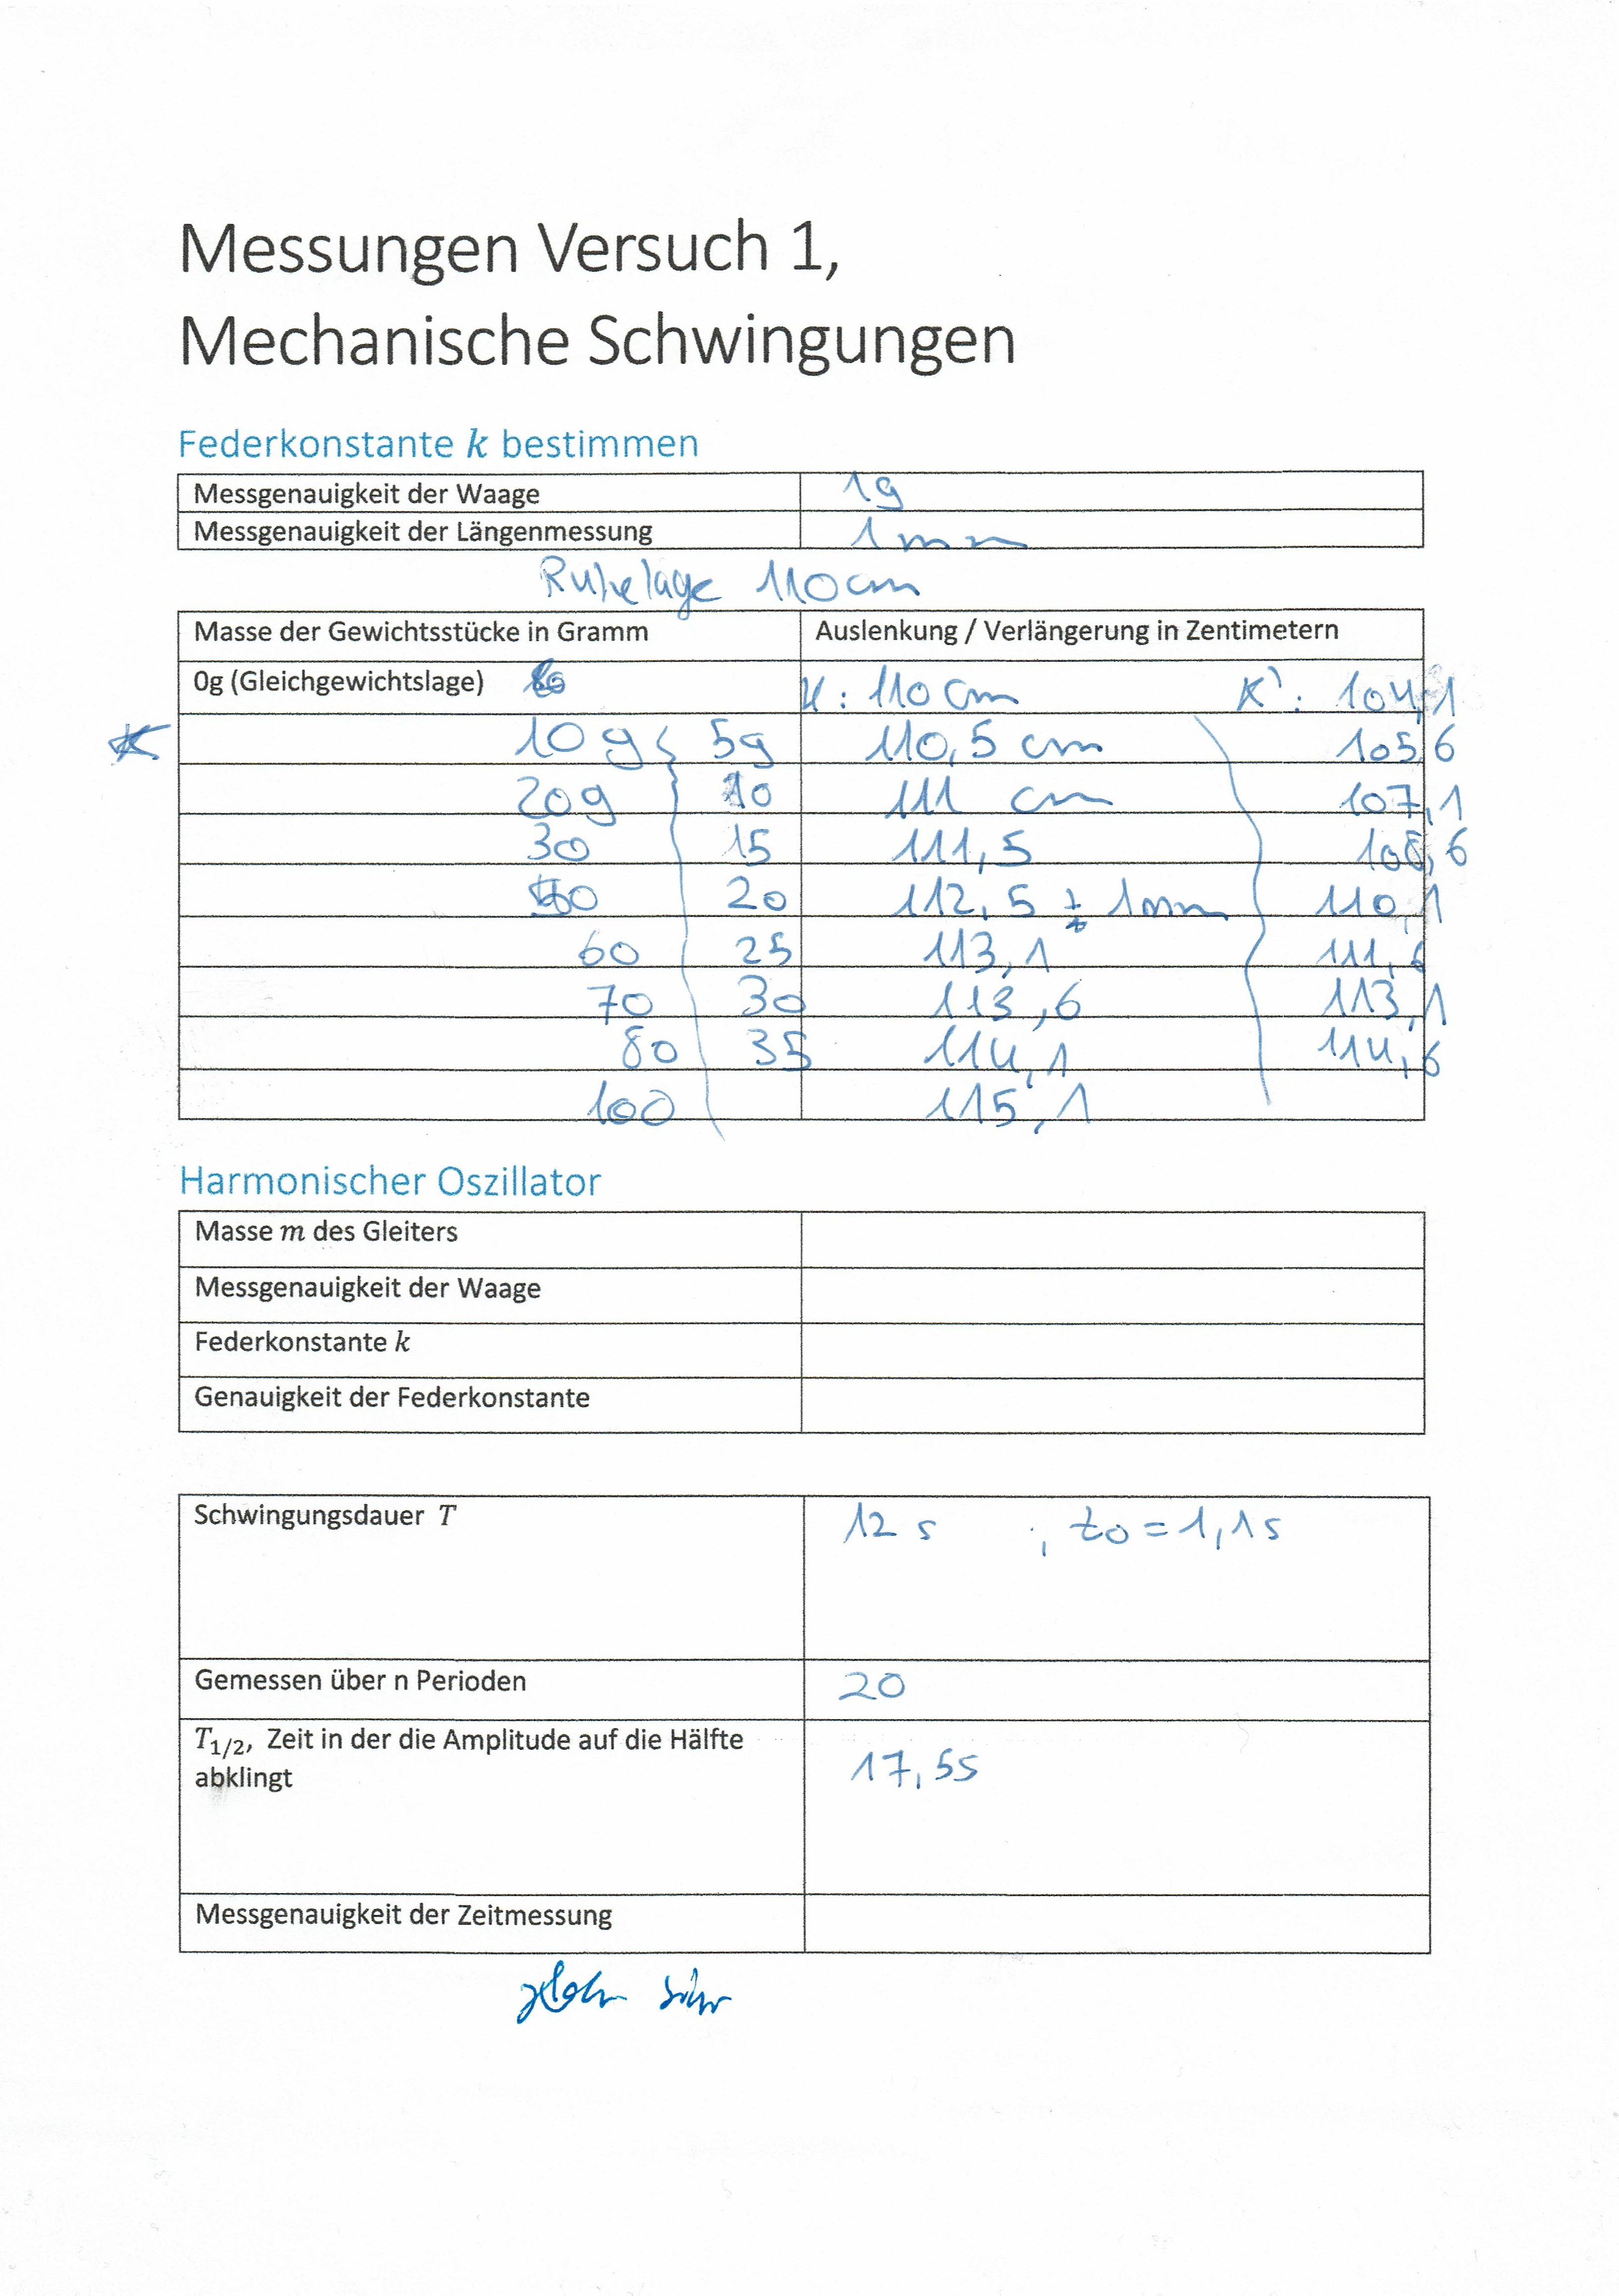
\includegraphics[height=14cm]{fotos/messwerte1_bild.jpg}
                  \caption{Messwerte der drei Versuchsdurchführungen}
              \end{figure}
              \begin{figure}[!ht]\label{fig:Messwerte2}
                  \centering
                  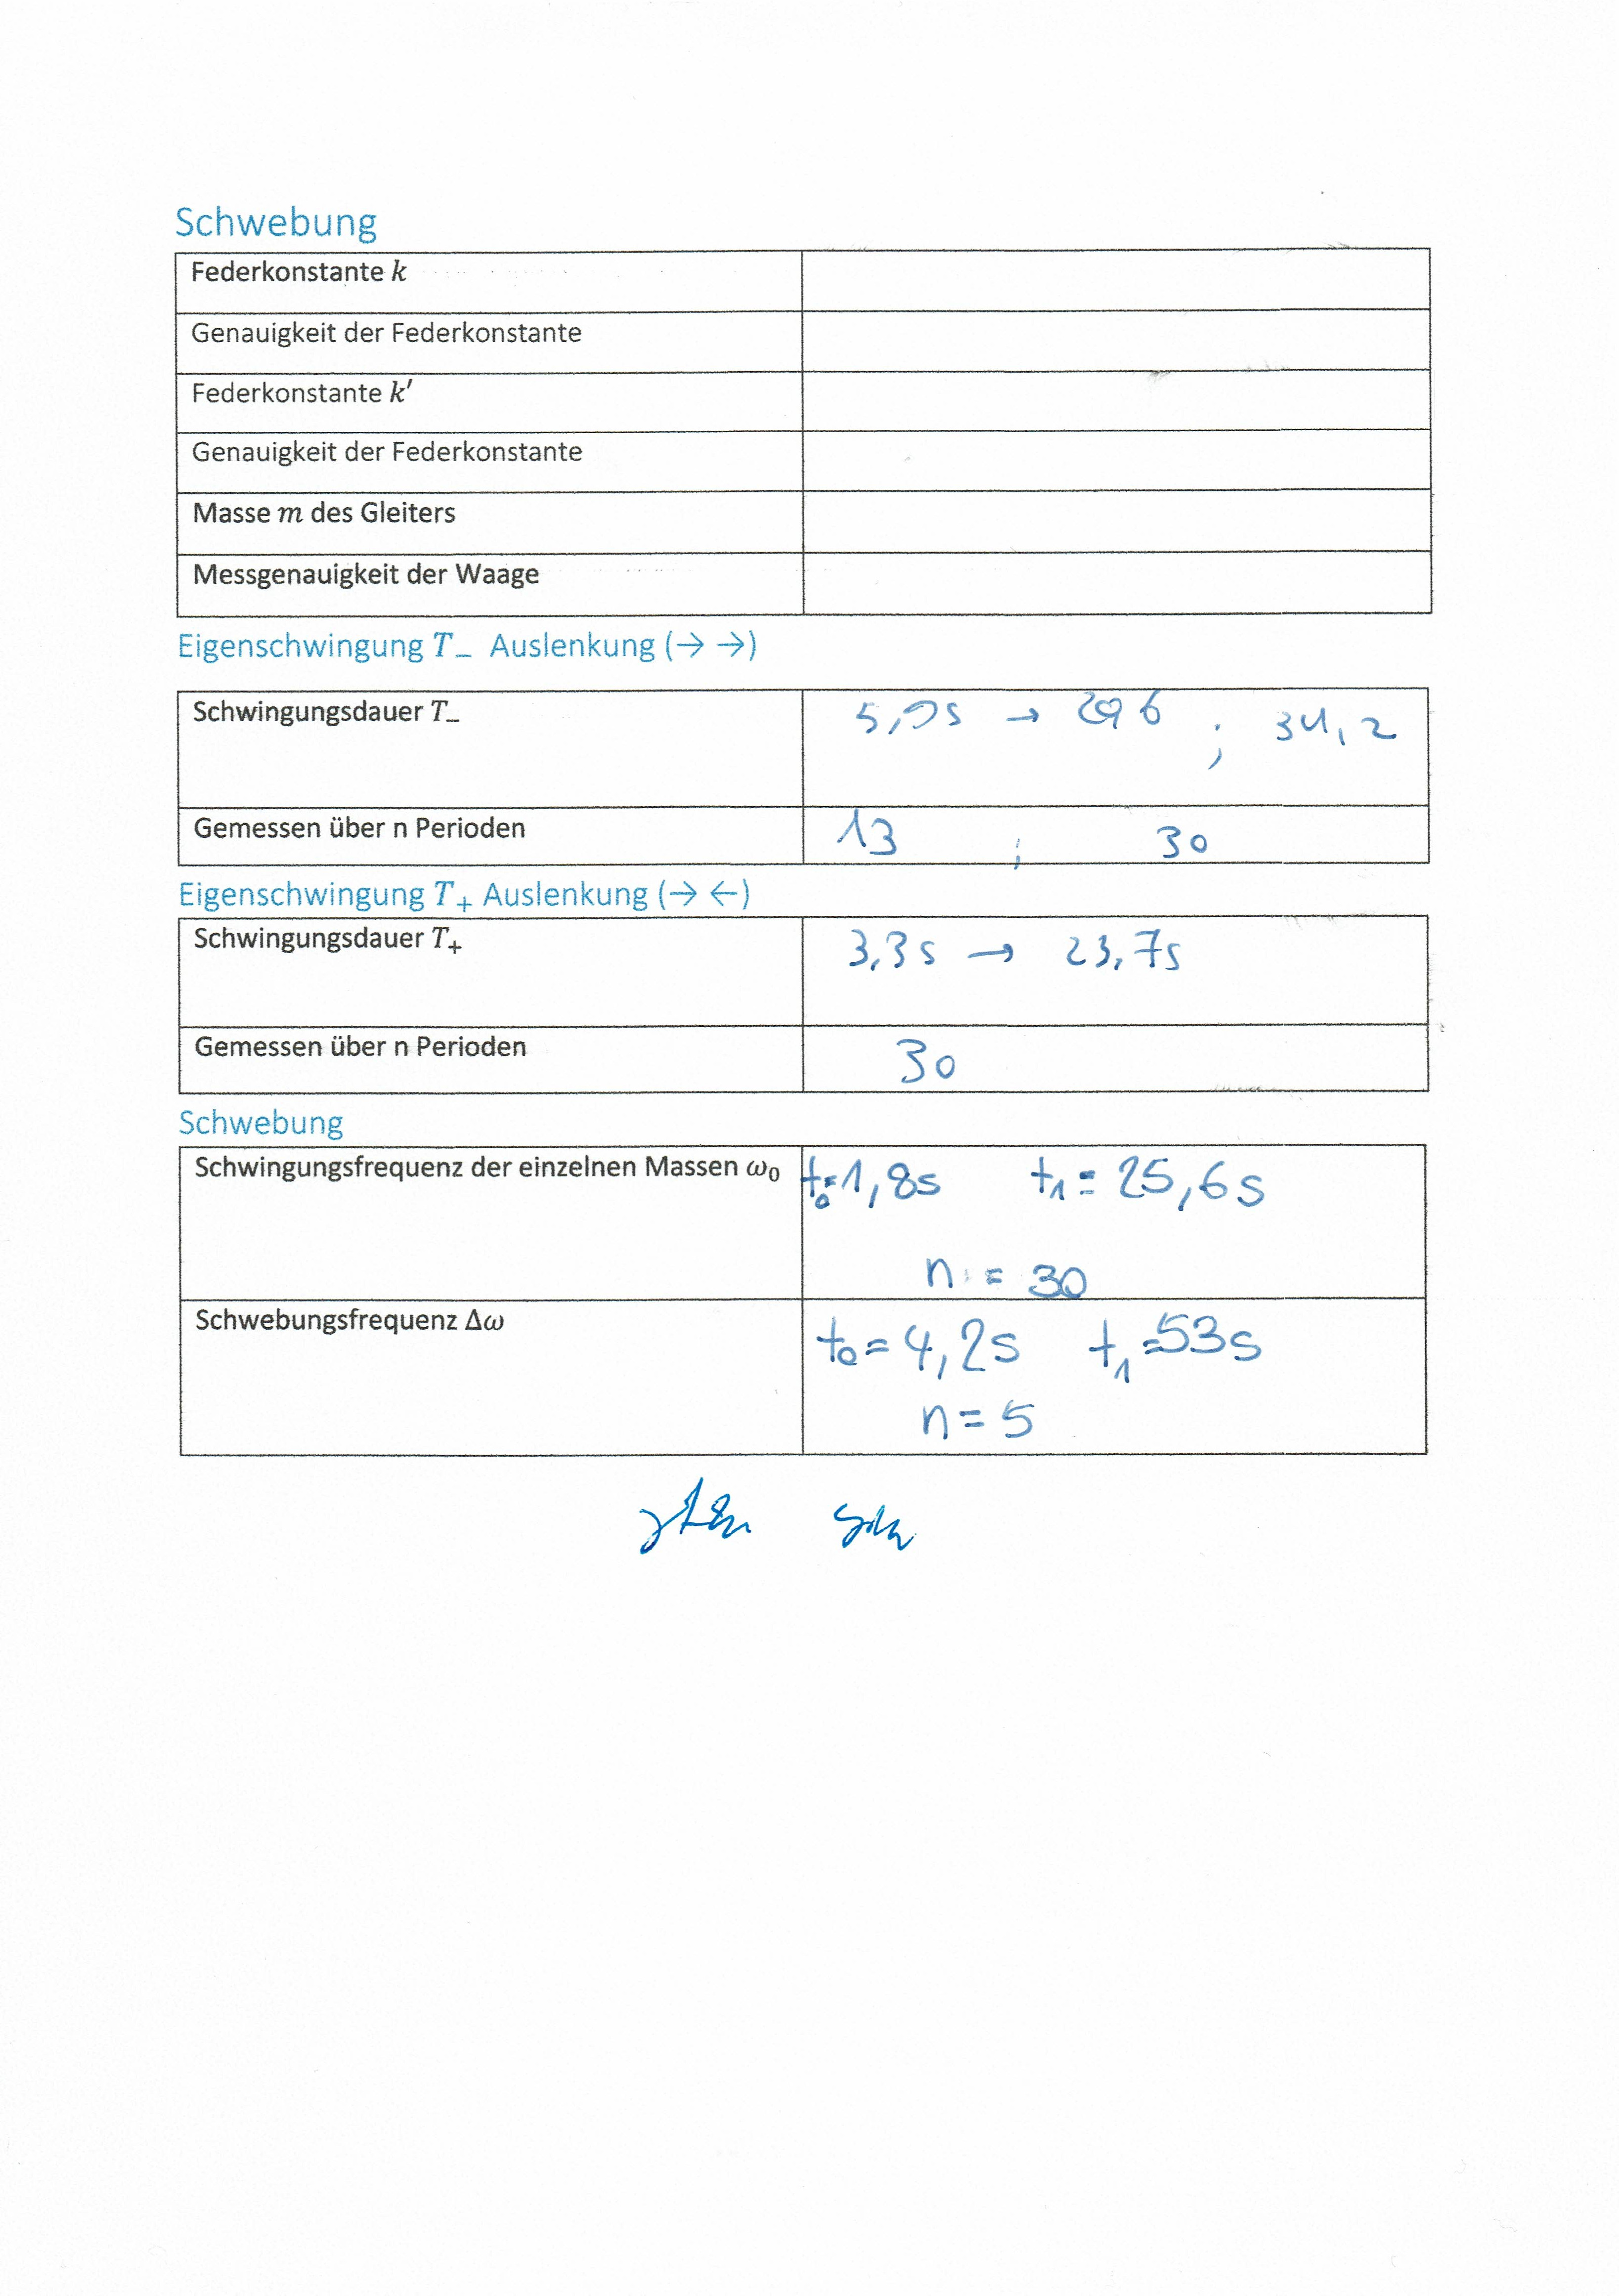
\includegraphics[height=14cm]{fotos/messwerte2_bild.jpg}
                  \caption{Messwerte der drei Versuchsdurchführungen}
              \end{figure}
              Die Messergebnisse für den Versuchsteil der Bestimmung der gleichphasigen Schwingung sind hier falsch eingetragen. Das erste verwendete Maximum ist erst bei \(t = \SI{9.9}{\second}\). Der Rest der Messwerte ist aber okay.

\section{Pythonskript zur Messdatenauswertung}
\begin{minted}{python}
import numpy as np
import matplotlib.pyplot as plt


def read_in_vcm(file_name, show_plot=False):
    # Read out vcm files
    path = f'../messdaten/{file_name}.vcm'

    with open(path, 'r') as file:
        # Skip file header
        for i in range(0, 22):
            file.readline()

        data_points = []

        # Read in data points from file
        value = file.readline().strip()
        while value == 'NAN' or value.count('.') == 0: 
            # Don't allow float which ends the the list
            if value != 'NAN':
                data_points.append(int(value))
            else:
                data_points.append('NAN')

            value = file.readline().strip()

        # generate x-Axis values with 0.1s intervals
        x_axis = [i/10 for i in range(0, len(data_points))]

        print(data_points.count('NAN'))

        # Remove 'NAN' values
        nan_times = 0
        for i in range(0, len(data_points) - data_points.count('NAN')):
            if data_points[i - nan_times] == 'NAN':
                data_points.pop(i - nan_times)
                x_axis.pop(i - nan_times)
                nan_times += 1

        if show_plot:
            plt.plot(x_axis, data_points)
            plt.show()

        return x_axis, data_points


def generate_csv(file_name, x_axis, data_points):
    # generate csv file
    path = f'../messdaten/{file_name}.csv'
    with open(path, 'w') as file:
        file.write('time, position \n')  # add header for pgfplots
        for i in range(0, len(data_points)):
            file.write(f'{x_axis[i]},{data_points[i]} \n')
        file.flush()


harmonisch = read_in_vcm('Versuch2')
gleich_phasig = read_in_vcm('Versuch3.1')
gegen_phasig = read_in_vcm('Versuch3.2')
schwebung = read_in_vcm('Versuch3.3')

# Write out in csv for loading with pgfplots
generate_csv('harmonisch', harmonisch[0], harmonisch[1])

# Exemplary usage for data analysis
data = np.array(gegen_phasig[1])
print(data.max())
print(data.mean())


\end{minted}

\end{document}